%
% 1. process this file with pdflatex
% 2. remind to process it twice otherwise cross-references will be wrong
%
\documentclass[a4paper,12pt]{article}
%
% This is to create hyperlinks for index, URLs and citations
% (now we can use the command \url{...} to create URL with hyperlink)
% 
\usepackage{color}
%
% For code and messages listings
\usepackage{listings}
%
\usepackage[a4paper,colorlinks=true,urlcolor=blue,citecolor=blue,linkcolor=blue,bookmarks=false,linktocpage]{hyperref}
%
% This allows inclusion of pictures.
% Create figures with PowerPoint and then export them individually
% in PDF, PNG, JPEG, or GIF format (in order of preference)
%
\usepackage[pdftex]{graphicx}
\DeclareGraphicsExtensions{.pdf,.png,.jpg,.gif}
%
% phantom space (for abbreviations)
%
\usepackage{xspace}
%
% Definition of margins
%
\usepackage[top=2cm,bottom=2cm,left=2cm,right=2cm]{geometry}
%
% This is needed if you write the report in Italian
%
%\usepackage[latin1]{inputenc}% IMPORTANTE! usare codifica ISO-8859-1 per le lettere accentate
%
% Paragraph skip and indent
%
\setlength\parskip{\medskipamount}
\setlength\parindent{0pt}
%
% Frequently used abbreviations.
%
\def\eg{e.g.\xspace}
\def\ie{i.e.\xspace}
\def\oauth{OAuth2\xspace}
\def\myfig#1{Fig.~#1\xspace}
\def\rfc#1{RFC-#1\xspace}

%
\begin{document}

\title{\oauth: protocol analysis and implementation
\\
{\normalsize Report for the Computer Security exam at the Politecnico di Torino}
}
\author{Luigi Ferrettino (254300)
\\
{\normalsize tutor: Dr.~Diana Berbecaru}
}
\date{July 2020}
\maketitle

\vfill

\rule{\textwidth}{1pt}
\newpage
\tableofcontents

\rule{\textwidth}{1pt}

\vfill

\newpage


% ------ SECTION 1 ------
\section{Introduction}
The present work aims at implementing a working demo complete solution that demonstrates the \oauth\ functionalities by analysing all the specification peculiarities, the security risks and its design downsides.

Open Authorization 2.0, more commonly called \oauth\, is an open communication protocol through which an application (or a web-service) can safely manage authorized access to sensitive data. The protocol is compatible with any type of application: desktop, web and mobile.
From a high level point of view, \oauth\ allows two parties to exchange securely and reliably sensitive information exploiting the concepts of \textit{federated identity} and \textit{delegated authority}. For example, some real-life scenarios are:

\begin{itemize}
    \item StackOverflow allowing you to log in with your Google account
    \item Posting a status update from your phone using the Facebook mobile application
    \item LinkedIn suggesting contacts for you to add by looking at your Google contacts
\end{itemize}

This protocol allows the creation of powerful applications that can all integrate with each other exchanging securely data and information.

An essential prerequisite in order to understand \oauth\ is the difference between \textit{authentication} and \textit{authorization}. This two terms might seem quite similar and sometimes they are interchanged, but actually they represent something totally different.
\textbf{Authentication} is the process of validating whether an actor (a person or a system) is really who it says it is or not.
As a real-life analogy, it could be useful to picture it as the act of showing the personal driver license to someone who wants to verify someone's identity (maybe when trying to access sensitive documents at the bank teller). 
This action could be recognised when the actor gives username and password to be \textit{authenticated} and retrieve a protected file or profile. 
\textbf{Authorization} instead, is the process of determining what actions someone can or cannot do once it is authenticated.
Coming back to the analogy of the bank teller, once that someone is authenticated and wants to do some actions, he needs authorization to do it and so he must pass both the authentication and authorization process in order to access, modify, delete some data. Usually this is implemented by looking up the permission in some access control lists.
Following these keywords, \oauth\ implements an \textit{authorization} protocol that could guarantees \textit{authentication} too when in conjunction to other ones (we will see more about it in the next sections).

In more practical terms, this protocol involves two different "common uses": the \textbf{federated identity} and the \textbf{delegated authority}.
The first one is a really important concept in the field of identity management. It pertains to the approach that allows one service provider (\ie\ Google) to allow authentication of a User using their identity with another service provider. As an example, Pinterest allowing Users to log in with their Google account.
Instead, the second one represents the ability of the service provider to gain access to User's resources from their behalf, like Facebook, which can suggest you to add contacts based on your Google (or a custom provider) ones; it is more or less a permission delegation.

In other words, the \oauth\ framework could provide both federated identity and delegated authority. It could, because strictly speaking it is only an authorization framework, so it doesn't support the federated identity. This is why a crucial importance is given by the third-part protocols that work in conjunction with it, like \textit{OIDC}\footnote{OpenID Connect, not to be confused with OpenID itself}, that provides an authentication layer on top of the \textit{\oauth} framework.
% ------ END SECTION 1 ------

% ------ SECTION 2 ------
\section{Protocol description}
After the first brief introduction, in this section the protocol will be described in details. \oauth\ has practically become the industry-standard one for authorization. Google, Facebook and other providers have a well documented API and a distributed access. Moreover, it is possible to implement a custom provider to use \oauth\ not as a social application, but for any kind of distributed system with unified access.

For what concerns the roles, there are in general four principal actors, described as follows:


\begin{itemize}
    \item The \textbf{Client}, acted by the application that is attempting to get access to the User's account (it needs to get permission from the User before doing it).
    \item The \textbf{Resource Server}, that implements the APIs to access the User's resources.
    \item The \textbf{Authorization Server}, that manages the authorizations delegation to the authenticated \oauth\ Client. It can be implemented alongside the Resource Server, as unique server, but for large-scale deployments it is usually separated.
    \item The \textbf{User} (Resource Owner) who is giving AuthZ to the Client to access personal information.
\end{itemize}

It is clear that they are mandatory for \oauth\ to work and they must be designed accordingly. 

% ------ SECTION 2.1 ------
\subsection{Introduction to the flows}
\label{section22}
In a generic use case, when someone has granted permission for an app in order to access his friend list on his behalf, it must happen an interaction between Facebook and the app itself. However, this interaction differs depending on the Client natures and capabilities: that is why \oauth\ supports various ways of exchanging information through the use of workflows.
In particular, using the adopted terminology, these are called \textit{grant types} and in the protocol can be found two main grant types that are used in the majority of the cases (the protocol specifies four grant types, but the other two ones are not used in real-world applications):

\begin{itemize}
    \item Implicit Grant
    \item AuthZ Code Grant
\end{itemize}

The first one is often cited as the \textbf{client-side workflow}, whereas the second one is often referred to as \textbf{server-side workflow}. To better understand these two workflows and their purposes, it is necessary to underline some key concepts.

% ------ SECTION 2.1.1 ------
\subsubsection{User consent}
When a Client wants to perform a particular action regarding someone or resources someone owns, it must first asks for \textit{permission}. If an App wants to access someone's friends list on Facebook, in order for Facebook to allow this, they must ask directly to the owner. This process may be familiar to many of us. For example, in \myfig{\ref{fig:usercon1}} we can see a screenshot of a User consent presented when someone wants to log into Pinterest using the Facebook credentials.

\vspace{0.5cm}
\begin{figure}[ht]
    \centering
    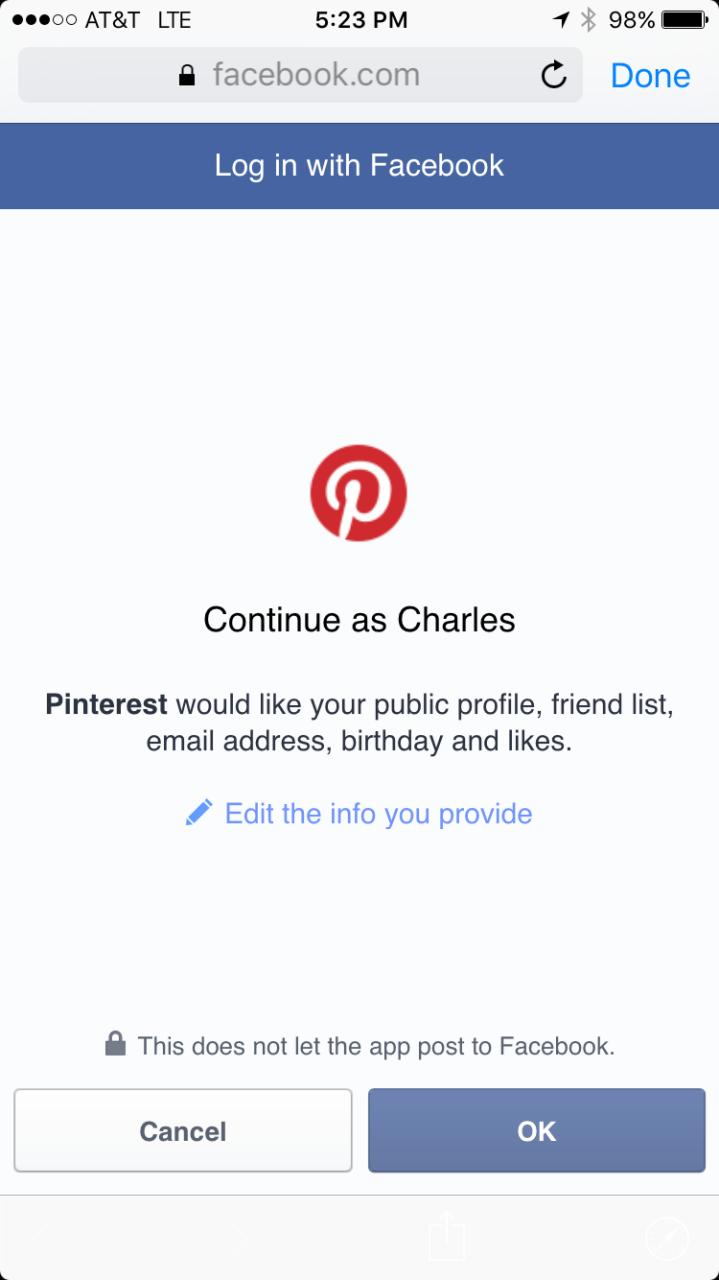
\includegraphics[width=0.4\textwidth]{figures/desktopaccess1.jpg}
    \caption{A classic User consent on Facebook}
    \label{fig:usercon1}
\end{figure}

A first draft of the flowchart sequence is presented in \myfig{\ref{fig:flow1}}. The simple steps are:

\begin{enumerate}
    \item The User asks App to suggest contacts.
    \item App says that to be done it needs the authorization here.
    \item App sends the User to Facebook. Here, Facebook asks him directly for authorization for App to access his friend list on his behalf. It does this by presenting the User consent form, which he can either accept or not. Let's assume he accepts.
    \item Facebook happily obliges, giving App the User's friend list. App then uses this information to tailor suggested contacts for him.
\end{enumerate}

However, it is necessary to specifically deal with the distinction of the two grant types in order to better integrate our concepts into a final flowchart.
% ------ END SECTION 2.1.1 ------

% ------ SECTION 2.1.2 ------
\subsubsection{Trusted/Untrusted Clients}

In \textit{\oauth} there are only two levels of trust: \textbf{confidential} and \textbf{public}. 
Therefore, a Client could be categorised into either of this trust levels following the two simple capabilities of storing and transmitting information securely.

A \textit{trusted Client} (\textbf{confidential}) is an application capable of storing and transmitting securely information (credentials, tokens, any other resources necessary for their application).
For example, it could be a 3-tier client-server-DBMS application where the back-end guarantees secure storage and transmission actions for confidential information. 

Instead, an \textit{untrusted Client} (\textbf{public}) is one which is incapable of doing such things and so they cannot be trusted on storing/transmitting securely the needed data. All browser-based applications are untrusted Clients (HTML/JS) because all the confidential data should be stored in the browser that is absolutely accessible by everyone.
It must be underlined that both capabilities of storing and transmitting must be fulfilled in order to call a Client \textit{trusted}.

When the User accepts this form, he has agreed to allow App to access to his Facebook friend list on his behalf. In simple terms, the User has delegated read-only authority to App for his Facebook friend list.
This workflow can be curated some more. There is a very important step in the
preceding process that requires a larger discussion. It is step 4 where App and
Facebook finally exchange the information that has been requested. In the previous diagram, it has been presented as a single step where Facebook gives the information to App. However, in reality, this is a much more complicated exchange that occurs, which depends on many factors.

\begin{figure}[ht]
    \centering
    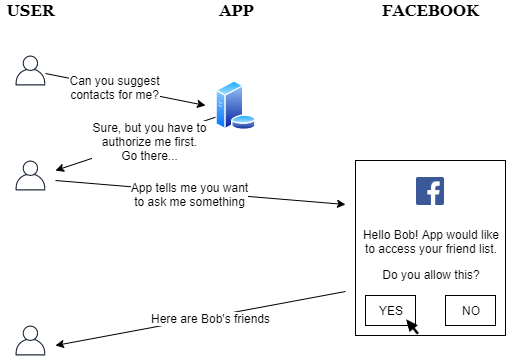
\includegraphics[width=0.9\textwidth]{figures/flow1.png}
    \caption{First draft of the flow}
    \label{fig:flow1}
    \vspace{0.5cm}
\end{figure}
% ------ END SECTION 2.1.2 ------

% ------ SECTION 2.1.3 ------
\subsubsection{Tokens and endpoints}
Tokens and endpoints are two important keywords of \oauth. In particular, a token is an abstraction that replaces that classic \textit{username} and \textit{password} with a single identifier that might have different formats, structures and methods of utilisation based on the server that implements it. 
The specification does not provide any information about the tokens format, but \oauth\ defines two types of token:

\begin{itemize}
    \item \textbf{Access Token}: a string that represents the authorization given to the Client. It is consumed by the Resource Server when a Client asks for a resource.

    \item \textbf{Refresh Token}: a particular family of tokens used to retrieve a new Access Token when the current one becomes invalid or expires. They are different from the classic ones because intended to be consumed only with AuthZ Servers (not Resource Servers).
\end{itemize}

Even if the Resource Server is an actor in the \oauth\ protocol, it is not an actor in the grant types, since the objective of the flows is to correctly issue an Access Token for the Client.

Furthermore, in Section 3 of the \rfc{6749}\ specification \cite{RFC6749}, \oauth\ defines three endpoints:

\begin{itemize}
    \item Authorization endpoint
    \item Token endpoint
    \item Redirection endpoint
\end{itemize}

Obviously, not every grant types defines the authorization endpoint and the token endpoint.

The \textbf{authorization endpoint} is used by the Client to obtain authorization from the User via User-agent redirection (the authorization server must first verify the identity of the User, \eg using OIDC) and it must use TLS\footnote{Transport Layer Security, "[...] cryptographic protocols designed to provide communications security over a computer network.". Source: \url{https://en.wikipedia.org/wiki/Transport_Layer_Security}} in order to have secure confidential data transmissions.

The \textbf{token endpoint} accepts requests from the Client in order to return an Access Token in exchange of an authorization code or a Refresh Token. This kind of endpoint is not used in the Implicit Grant Type flow (see section \ref{section22}), because in this case the token is issued directly.

Finally, the \textbf{redirection endpoint} is used by the AuthZ Server to redirect the User back to the Client. The authorized redirection endpoints must be known by the AuthZ Server in order to avoid some kinds of attacks.
% ------ END SECTION 2.1.3 ------
% ------ END SECTION 2.1 ------

% ------ SECTION 2.2 ------
\subsection{Client-side flow (untrusted)}
The Implicit Grant flow is optimised for scripting language based Clients (web applications running on the browser). As a result of the User authorization, the Client is issued directly an Access Token. This flow is defined in Section 4.2 of the \rfc{6749}\ \cite{RFC6749}. It is important to say that, when using this flow, the AuthZ Server does not authenticate the Client. 

In this flow, the User-agent is the main actor, since it is the web-browser and it interacts directly with both the User (Resource Owner) and the Client (a web-app that is running on the User-agent) while redirecting. The Hosted Resource is a local or remote entity that often returns an HTML page with a JavaScript source used by the User-agent in order to extract the Access Token from the Token response of the AuthZ Server. In the \myfig{\ref{fig:flowa}} is shown a general schema of the flow. The steps follows:

\begin{figure}[htbp]
    \centering
    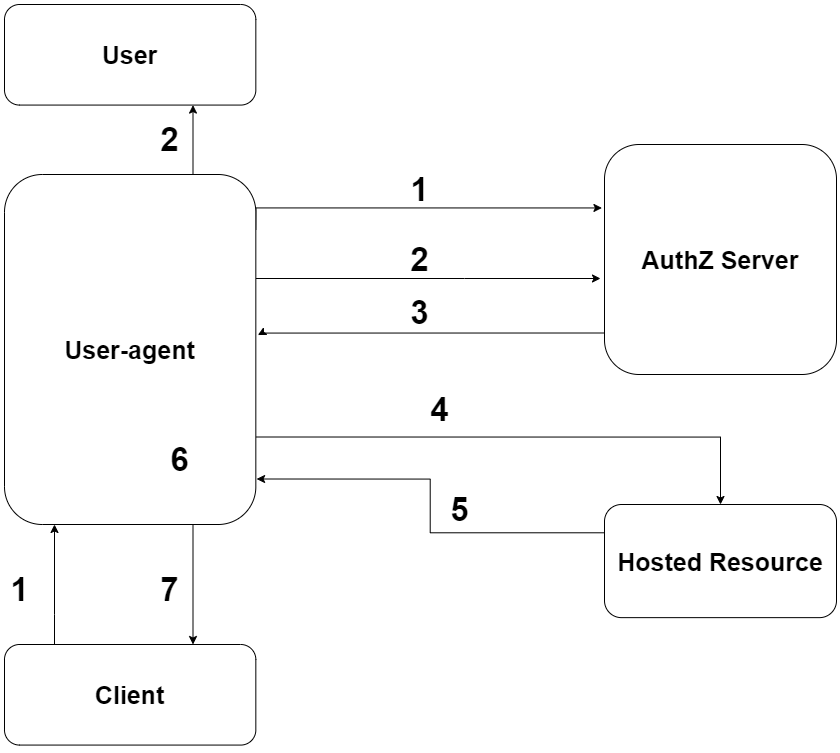
\includegraphics[width=0.7\textwidth]{figures/implicit_flow_general.png}
    \caption{Implicit Grant flow}
    \label{fig:flowa}
\end{figure}

\label{step1implicit}
\begin{enumerate}
    \item The User-agent redirects to the URI built by the Client according to the specification. This URI is created by adding some parameters into the URI fragment encoded in the \textit{application/x-www-form-urlencoded} format. A valid authorization request is:

    \begin{lstlisting}[basicstyle=\ttfamily]
      GET /authorize?
        response_type=token&
        client_id=[client_id]&
        redirect_uri=[redirect_uri]&
        scope=[scope]&
        state=[state] HTTP/1.1
      Host: server.example.com
    \end{lstlisting}
    
    \item The User-agent will present to the User (that is currently looking at the User-agent) the User consent page on \url{http://server.example.com/authorize} (on the AuthZ Server). Here, the User logs into his account on the AuthZ Server and accepts the authorization consent.
    
    \item If all the parameters are valid, the AuthZ Server builds an HTTP 302 Found response with the previously received \texttt{redirect\_uri} adding the Access Token and other parameters in the URI fragment. The AuthZ Server inserts the complete \texttt{redirect\_uri} in the \texttt{Location} header. The Token response is sent:
    
    \begin{lstlisting}[basicstyle=\ttfamily]
      HTTP/1.1 302 Found
        Location: [redirect_uri]#
        access_token=[access_token]&
        token_type=[token_type]&
        expires_in=[expires_in]&
        scope=[scope]&
        state=[state]
    \end{lstlisting}
    
    \item When the User-agent encounters an HTTP 302 Found, it redirects immediately to the specified URI in the \texttt{Location} header, but without the URI fragment that is not sent across the network. The \texttt{redirect\_uri} often points to an HTML page hosted locally or remotely (Hosted Resource) that contains the script that will correctly pass the Access Token and the other parameters to the Client. This mechanism is implemented for security reasons: it prevents the User-agent to run any malicious script during the redirection time. Only the script returned by the HTML page is considered trustworthy.
    
    \item The Hosted Resource (\eg\ and HTML page with an embedded script) is returned and rendered by the User-agent.
    
    \item  The User-agent runs the script in order to extract all the parameters from the URI fragment of the step 3.
    
    \item Finally, the Client receives the Access Token and all the parameters by the executed script.
\end{enumerate}

The Implicit Grant flow is much faster and simpler than any other Grant Type and it is well suited for a simple web-app without any back-end server. This flexibility comes with many security issues, starting from the public availability of the Access Token, that is locally available in the User-agent and it can be extracted by any dangerous script.

% ------ SECTION 2.2.1 ------
\subsubsection{Analysis of the exchanged messages}
At this point, it is clear that for what concerns the Implicit Grant flow we have only an \textbf{authorization request} and an \textbf{Token response}. Both of them must be encoded accordingly to the specification into the endpoint URI in the \textit{application/x-www-form-urlencoded} format.

\paragraph{Authorization request}
\label{authreq}
With respect to \myfig{\ref{fig:flowa}}, the authorization request is done in step 1.
The Client MUST build this request using these parameters into the URI fragment:

\texttt{response\_type}

\hspace{0.5cm}REQUIRED. The type has to be \textit{token}.

\texttt{client\_id}

\hspace{0.5cm}REQUIRED. This value must be set with the application's unique client\_ID.

\texttt{redirect\_uri}

\hspace{0.5cm}OPTIONAL. This value could be set with the URI of the redirection endpoint used by 

\hspace{0.5cm}the service provider to return the response, whether that is an Access Token in 

\hspace{0.5cm}the case of a successful request, or an error message in the case of a failed request.

\texttt{scope}

\hspace{0.5cm}OPTIONAL. The scope of permissions that we are requesting on behalf of the User.

\texttt{state}

\hspace{0.5cm}RECOMMENDED. String issued by the Client in order to maintain a state with

\hspace{0.5cm}the response. Value used by the AuthZ Server to redirect the User-agent back to

\hspace{0.5cm}the Client.As it will be shown in the following sections, the parameter should be

\hspace{0.5cm}used to avoid CSRF\footnote{Cross-site request forgery, "[...] when a malicious program causes a User's web browser to perform an unwanted action on a trusted site on which the User is currently authenticated.". Source: \url{https://auth0.com/docs/protocols/oauth2/mitigate-csrf-attacks}}.


\paragraph{Error response}
\label{tokenerr}
It could happen that the AuthZ Server returns an error message (\eg\ the User consent is rejected by the User itself). In this case, an error message is built with those parameters in the fragment of the URI of redirection:

\texttt{error}

\hspace{0.5cm}REQUIRED. Single ASCII code representing the error:

\begin{itemize}
\item[] \begin{itemize}
        \item \texttt{invalid\_request}
        \item \texttt{unauthorized\_client}
        \item \texttt{access\_denied}
        \item \texttt{unsupported\_response\_type}
        \item \texttt{invalid\_scope}
        \item \texttt{server\_error}
        \item \texttt{temporarily\_unavailable}
\end{itemize}
\end{itemize}

\texttt{error\_description}

\hspace{0.5cm}OPTIONAL. Human-readable message describing what caused the error.

\texttt{error\_uri}

\hspace{0.5cm}OPTIONAL. Link to more information about the error.

\texttt{state}

\hspace{0.5cm}REQUIRED. If a state parameter was present in the request.

\vspace{0.5cm}

\noindent An example of an error response is:

\begin{lstlisting}[basicstyle=\ttfamily]
  HTTP/1.1 302 Found
    Location: [redirect_uri]#
    error=[error_code]&
    error_description=[error_description]&
    error_uri=[error_uri]&
    state=[state]
\end{lstlisting}

It is important to notice the HTTP 302 Found that redirects to the \texttt{Location} header value. In \myfig{\ref{fig:flowa}}, this error response could be returned in step 3.

\paragraph{Token response}
When the provider grants the access request, according to the specification it sends a positive response adding to the fragment component of the redirection URI in the \textit{application/x-www-form-urlencoded} format the following parameters:

\texttt{access\_token}

\hspace{0.5cm}REQUIRED. It is this token value that we will eventually use to access

\hspace{0.5cm}the User's profile and feed data.

\texttt{token\_type}

\hspace{0.5cm}REQUIRED. As it suggests, specifies the type of token used

\hspace{0.5cm}to make a protected resource request.

\texttt{expires\_in}

\hspace{0.5cm}RECOMMENDED. The lifetime of the token in seconds. It could not be

\hspace{0.5cm}returned by the server.

\texttt{scope}

\hspace{0.5cm}REQUIRED. The scopes of the Access Token.

\hspace{0.5cm}OPTIONAL. If they are the same requested by the Client.

\texttt{state}

\hspace{0.5cm}REQUIRED. If a state parameter was present in the request.

% ------ END SECTION 2.2.1 ------
% ------ END SECTION 2.2 ------

% ------ SECTION 2.3 ------

\subsection{Server-side flow (trusted)}
\label{authcg}

The AuthZ Code Grant is the most used grant type and it is built for Client confidentiality thanks to the \textit{trusted} capability of a web-server that implements it. With respect to the Implicit Grant flow, the Client is now a fully functional web-server (\ie\ a server capable of storing, processing and delivering web pages). The name of this grant type refers to a temporary string called "code" (the AuthZ Code), issued by the AuthZ Server, that represents the accepted authorizations of the User. This AuthZ Code will be later consumed by the Client in exchange of the Access Token. Another difference with respect to the Implicit Grant flow is that the Client must be manually registered on the AuthZ Server (\ie\ the AuthZ Server permanently stores \texttt{client\_id} and \texttt{client\_secret} for each possible Client) in order to implement the \textit{Client authentication}. 

\begin{figure}[ht]
    \centering
    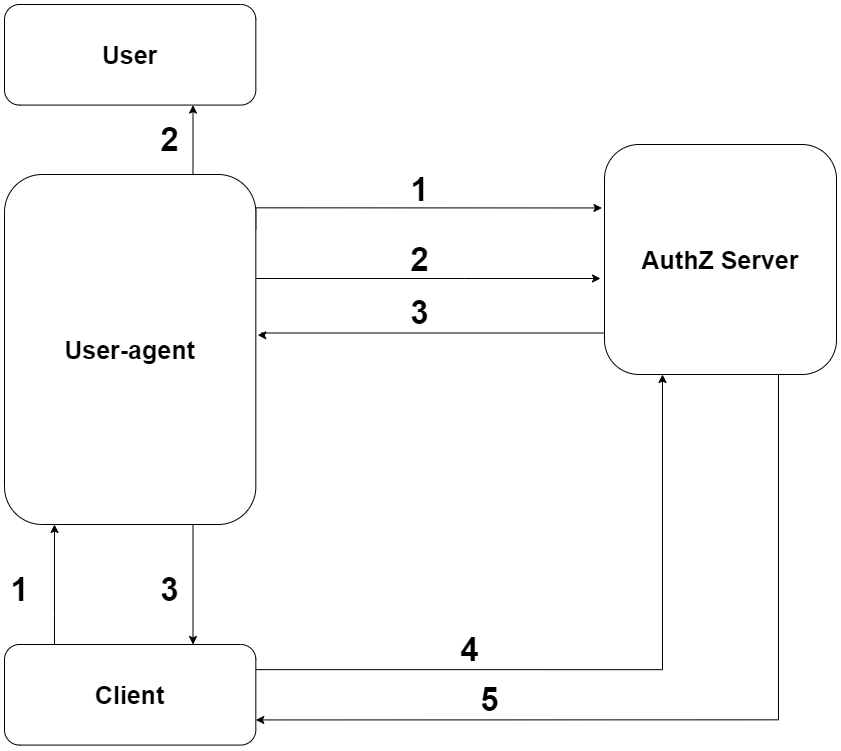
\includegraphics[width=0.7\textwidth]{figures/server_flow_general.png}
    \caption{AuthZ Code Grant flow}
    \label{fig:serverflow}
\end{figure}

This flow is described in Section 4.1 of the \rfc{6749}\ \cite{RFC6749}. Moreover, this flow enables the Refresh Token flow that can be used to update the Access Token when it expires, without the User intervention. In \myfig{\ref{fig:serverflow}} is provided a general description of this flow:



\begin{enumerate}
    \item The flow starts with the Client that builds the same URI with the same parameters as in step 1 of the Implicit Grant flow (see \ref{step1implicit}) and redirects the User on the AuthZ Server dedicated endpoint. The only difference with respect to the Implicit Grant flow is the parameter \texttt{response\_type} MUST be set to "code". The authorization request is built as follows:
    
    \begin{lstlisting}[basicstyle=\ttfamily]
      GET /authorize?
        response_type=code&
        client_id=[client_id]&
        redirect_uri=[redirect_uri]&
        scope=[scope]&
        state=[state] HTTP/1.1
      Host: server.example.com
    \end{lstlisting}
    
    \item The User-agent will present to the User (that is currently looking at the User-agent) the User consent page on \url{http://server.example.com/authorize} (on the AuthZ Server). Here, the User logs into his account on the AuthZ Server and accepts the authorization consent. This step is equal to the same step of the Implicit Grant flow.
    
    \item If all the parameters are valid, the AuthZ Server builds an HTTP 302 Found response with the previously received \texttt{redirect\_uri} adding the AuthZ Code and other parameters in the query component (as opposed to the Implicit Grant, where the parameters are formatted into the URI fragment).  The AuthZ Server inserts the complete \texttt{redirect\_uri} in the \texttt{Location} header and builds the authorization response:
    
    \begin{lstlisting}[basicstyle=\ttfamily]
      HTTP/1.1 302 Found
        Location: [redirect_uri]?
        code=[authorization_code]&
        state=[state]
    \end{lstlisting}
    
    \item When the User-agent encounters an HTTP 302 Found,  it redirects immediately to the specified URI in the \texttt{Location} header. With respect to the Implicit Grant flow, now the parameters are in the query component, thus they are passed to the \texttt{redirect\_URI}. This URI is often an endpoint of the Client (since, as already mentioned, it is a web-server too). The Client checks the validity of the parameters and saves the AuthZ Code.
    
    \item Without any interaction with the User nor the User-agent, the Client prepares a Token request directly on a dedicated endpoint \url{http://server.example.com/token} of the AuthZ Server by using an HTTP POST:
    
    \begin{lstlisting}[basicstyle=\ttfamily]
      POST /token HTTP/1.1
      Host: server.example.com
      Authorization: Basic [base64url_encoded_client_secrets]
      Content-Type: application/x-www-form-urlencoded
    
      grant_type=authorization_code&
        code=[authorization_code]&
        redirect_uri=[redirect_uri]&
        client_id=[client_id]
    \end{lstlisting}
    
    As already mentioned before, in order to pass these parameters the Client application must also identify itself with the AuthZ Server. This is an added layer of security (only necessary for trusted Clients) and it is known as \textit{Client
    authentication}. It entails the secure transmission of the Client credentials to the AuthZ Server for validation. It must be pointed out that although the \oauth\ specification doesn't specify any particular authentication scheme for Client authentication, this is typically done using HTTP basic authentication (defined in \rfc{2617}).
    In other words, it is the Base64-encoded value of the Client credentials in
    the form:

    \quad \texttt{BASE64URL([client\_id]:[client\_secret])} 
    
    That is added into the \texttt{Authorization} header.
    
    The \texttt{grant\_type} parameter MUST be set to "authorization\_code", since the AuthZ Server has to know the kind of request.
    
    The \texttt{redirect\_uri} is often different from the previous one, since it refers to another endpoint of the Client that is waiting for the future Access Token.
    
    \item The AuthZ Server checks the Token request and if everything is correct, generates a new Access Token (and SHOULD generate a Refresh Token too) and sends the Token response to the specified \texttt{redirect\_uri} of the Client:
    
    \begin{lstlisting}[basicstyle=\ttfamily]
      HTTP/1.1 200 OK
      Content-Type: application/json;charset=UTF-8
      Cache-Control: no-store
      Pragma: no-cache
      {
        "access_token":"2YotnFZFEjr1zCsicMWpAA",
        "token_type":"bearer",
        "expires_in":3600,
        "refresh_token":"tGzv3JOkF0XG5Qx2TlKWIA",
      }
    \end{lstlisting}    
    
    The most used format for the Token response is the JSON format. The Client now has the Access Token and the Refresh Token.
    
\end{enumerate}


With the AuthZ Code Grant flow, since the Client is a \textit{trusted} application capable of storing and transmitting the token securely, some security issues of the Implicit Grant flow disappear. So, naturally, this Client confidentiality comes at a price: complexity. There are twice as much messages exchanged with respect to the Implicit Grant flow, much more libraries to integrate in the code and more parameters to manage. Nevertheless, this is the recommended flow and other flows must be used only in particular cases.

% ------ SECTION 2.3.1 ------
\subsubsection{Analysis of exchanged messages}
The exchanged messages flow is more complex now. Throughout the AuthZ Code Grant flow, two more messages that precede the Token request and response are added: the \textbf{authorization request} and the \textbf{authorization response}. Furthermore, it is suggested the Token Refresh flow use.

\paragraph{Authorization request}
According to the specification, this request is the one to gain consent from the User. This message is nearly identical to the authorization request made in the previous section for the Implicit Grant flow (\ref{authreq}), except for one important difference: the value of the \texttt{response\_type} parameter MUST be set to "code" instead of "token".

\noindent This message, with respect to the \myfig{\ref{fig:serverflow}}, is exchanged during step 1. 

\paragraph{Authorization response}
If the request URL is correctly formatted and constructed, the AuthZ Server will send back a response. If the response will be positive, an authorization code is sent in order to be afterwards converted in an Access Token.
The possible parameters that can be expected in the preceding response are now in the query component and not in the fragment one:

\texttt{code}

\hspace{0.5cm}REQUIRED. AuthZ code to be exchanged.

\texttt{state}

\hspace{0.5cm}REQUIRED. If a state parameter was present in the request.

\vspace{0.5cm}

\noindent This message, with respect to the \myfig{\ref{fig:serverflow}}, is exchanged during step 3. 

\vspace{0.5cm}

On the other hand, if the response will be negative, the error will be built as in the Implicit Grant flow (same properties as in \ref{tokenerr}). The difference relies only in the fact that it is returned in the query component instead of the fragment one.

This message, with respect to the \myfig{\ref{fig:serverflow}}, is exchanged during step 3. An example of valid authorization error response is:

\begin{lstlisting}[basicstyle=\ttfamily]
  HTTP/1.1 302 Found
    Location: [redirect_uri]?
    error=[error_code]&
    error_description=[error_description]&
    error_uri=[error_uri]&
    state=[state]
\end{lstlisting}

\paragraph{Token request}
Once that the authorization code has been retrieved, it can be used to exchange an Access Token. With this objective, the Client makes a request by using an HTTP POST, specifying in the body section the following parameters:

\texttt{grant\_type}

\hspace{0.5cm}REQUIRED. The value MUST be "authorization\_code".

\texttt{code}

\hspace{0.5cm}REQUIRED. It MUST be set to the value of the previously retrieved

\hspace{0.5cm}authorization code

\texttt{redirect\_uri}

\hspace{0.5cm}REQUIRED. If a redirect\_uri parameter was present in the request.

\texttt{client\_id}

\hspace{0.5cm}REQUIRED. The application unique client\_ID.

\vspace{0.5cm}

\noindent This message, with respect to the \myfig{\ref{fig:serverflow}}, is exchanged during step 3. 


\paragraph{Token response}
As it has been encountered in the previous responses, if the authorization code is valid, we will get our Access Token or an error otherwise. Depending on the implemented AuthZ Server, we could possibly get an optional Refresh Token (\ref{accref}) in order to update our expired Access Token without doing all the previous steps.

For a \textbf{success} response it is sent back a message with the following parameters in the entity-body (e.g.in JSON):

\texttt{access\_token}

\hspace{0.5cm}REQUIRED. It contains the token: successful authorization and Token request! 

\texttt{token\_type}

\hspace{0.5cm}REQUIRED. Defines the type of token sent.

\hspace{0.5cm}In almost all of the cases this will be \textit{bearer}.

\texttt{expires\_in}

\hspace{0.5cm}RECOMMENDED. The time-to-live of the token.

\hspace{0.5cm}If this value is 7200, that means that the Access Token will expire

\hspace{0.5cm}two hours from the time the response message was generated.

\vspace{0.5cm}

\texttt{refresh\_token}

\hspace{0.5cm}OPTIONAL. It may be used to refresh the Access Token in case it expires.

\texttt{scope}

\hspace{0.5cm}REQUIRED. The authorized scopes of the Access Token.

\hspace{0.5cm}OPTIONAL. If they are the same requested by the Client.

\vspace{0.5cm}

This message, with respect to the \myfig{\ref{fig:serverflow}}, is exchanged during step 6.

The specification does not provide any information about the type of Access Token (and Refresh Token), that is why it can be a generic string. Nevertheless, JSON Web Token (JWT) [\rfc{7519}] \cite{RFC7519} is one of the most used. 
% ------ END SECTION 2.3.1 ------

% ------ SECTION 2.3.2 ------
\subsubsection{Refresh Token Flow}
\label{accref}
The AuthZ Code Grant flow SHOULD implement the Refresh Token flow. By using the Refresh Token, the Client (with the AuthZ Server) reduces the User interactions requested by the flow itself:  when the Access Token expires, the User must actively participate to the AuthZ Code Grant by manually accepting all the authorization requests again and again. In order to avoid this, the Refresh Token allows to be exchanged with a new Access Token for the original authorization scopes, reducing the active User interaction only when new authorization scopes are requested.  In \myfig{\ref{fig:refreshtok}} is shown a the basic flow:

\begin{enumerate}
    \item Supposing that the AuthZ Code Grant flow was already performed and the Client has a valid Refresh Token, in this step the Client performs a normal request to the Resource Server using his Access Token:
    
    \begin{lstlisting}[basicstyle=\ttfamily]
    GET /resource HTTP/1.1
    Host: resource.example.com
    Authorization: Bearer [access-token]
    \end{lstlisting}
    
    
    \item The Resource Server checks the Access Token and validates it, discovering that it is expired. It prepares an error Token response by specifying in the \texttt{error\_description} that the Access Token is expired:
    
    \begin{lstlisting}[basicstyle=\ttfamily]
    HTTP/1.1 401 Unauthorized
    WWW-Authenticate: Bearer error="invalid_token"
    error_description="The Access Token expired"
    Content-type: application/json
 
    {
      "error": "invalid_token",
      "error_description": "The Access Token expired"
    }
    \end{lstlisting}
    
    \item When the Client receives and extract the error, this is were the Refresh Token flow starts. The Client prepares and sends a Token request by using the Refresh Token (that, in a way, substitutes the AuthZ Code in the AuthZ Code Grant flow, but without the User intervention).
    
    \begin{lstlisting}[basicstyle=\ttfamily]
    POST /token HTTP/1.1
    Host: server.authz.com
    Authorization: Basic [base64url_encoded_client_credentials]
    Content-Type: application/x-www-form-urlencoded
    
    grant_type=refresh_token&refresh_token=[refresh_token]
    \end{lstlisting}
    
    
    \item The AuthZ Server receives the request and knows what to expect because the \texttt{grant\_type} parameter is set to "refresh\_token". It validates the Refresh Token, generates and sends a new Access Token and Refresh Token for the original scopes.
    
    \begin{lstlisting}[basicstyle=\ttfamily]
    HTTP/1.1 200 OK
    Content-Type: application/json;charset=UTF-8
    Cache-Control: no-store
    Pragma: no-cache
    
    {
      "access_token":"2YotnFZFEjr1zCsicMWpAA",
      "token_type":"bearer",
      "expires_in":3600,
      "refresh_token":"tGzv3JOkF0XG5Qx2TlKWIA"
    }
    \end{lstlisting}
    
    \item The Client receives both the tokens and uses the Access Token to perform the resource request.
    \item The Resource Server validates the Access Token and returns the requested resource. 
\end{enumerate}

\begin{figure}[ht]
    \centering
    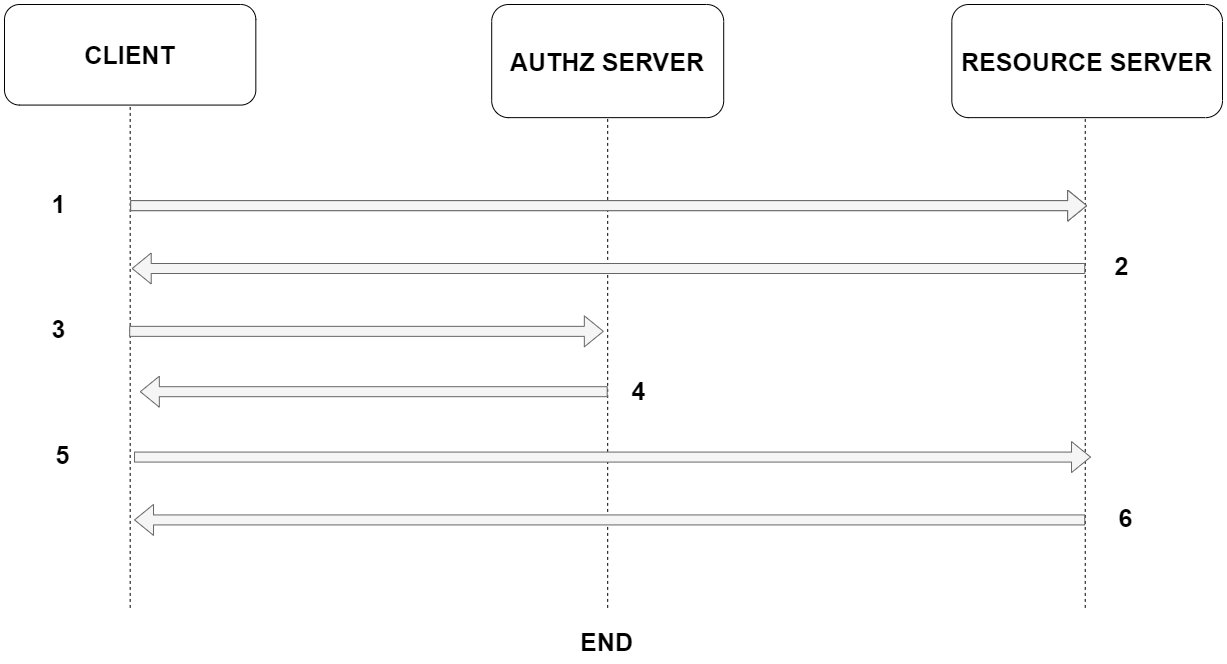
\includegraphics[width=\textwidth]{figures/refresh_token_general.png}
    \caption{Refresh Token flow}
    \label{fig:refreshtok}
\end{figure}


It must be noticed that during the Refresh Token flow, a new Refresh Token too is given. That is because even the Refresh Token has an expiration (normally longer than the Access Token).
Furthermore, the Resource Server is strictly not an actor of the flow, but here is used in order to explain how the Refresh Token flow is started by the Client (\ie\ the action that triggers the flow to start).
% ------ END SECTION 2.3.2 ------
% ------ END SECTION 2.3 ------

% ------ SECTION 2.4 ------
\subsection{About mobile applications}
Typically, when someone talks about \textit{mobile application}, he is referring to one of the two types of applications:

\begin{itemize}
    \item Mobile-optimised web application
    \item Native mobile application
\end{itemize}

The first one is nothing more than a customised browser that runs the web app optimised for the small screen. Since that, the same rules as a desktop web browser are applied.
The second one though, is a natively installed mobile app, an entirely new platform developed in recent years. For this last type, what flow should be used? 

In order to answer this question, just as developing other types of Client apps, the flow to be used is based on whether the platform is suitable for being trusted or not. In order for a mobile application to be considered trusted, it must be able to securely store and transmit confidential information. This can really only be achieved in
one way, with the use of a back-end server. If a mobile application has a back-end server that powers it, this server can also be used to securely store and transmit any confidential information it needs to. In this case, yes, this particular type of mobile application can be considered trusted, and should therefore use the AuthZ Code Grant flow (as for a web application with a server). 

In the absence of it though, the application will be unable to securely store and transmit confidential information, and cannot be considered trusted. In this scenario, the mobile application should use the Implicit Grant flow (as for a standalone web app).

% ------ SECTION 2.4.1 ------
\subsubsection{Secure storage APIs}
It is quite common that not all mobile applications are powered by a back-end server. Rather than use the Implicit Grant flow, there is a solution that can still archive secure (not strictly) storage capabilities by exploiting secure storage APIs in some mobile platforms like iOS and Android.  For the most part, this is enough for most applications to be considered trusted. Client credentials can be stored here and they can communicate directly with the service provider through the application, accessing these secrets via the APIs without the use of a back-end server.

However, strictly speaking, this is not considered trusted. It is true that the confidential data is encrypted, but it is accessible by the attacker. Data and User/attacker are in the same \textit{space} using this method, while with a back-end server the so called User/attacker space is external with respect to the storage services and not accessible. The platform's secure storage APIs may well be extremely secure and difficult for attackers to break, but in strict terms it is possible and, in the world of security, \textit{possible} should be assumed as \textit{probable}. This is why mobile applications that do not have back-end servers, but make use of the mobile platform's secure storage APIs, should not be considered trusted and should therefore not use the AuthZ Code Grant flow.

Since the architecture of the mobile application can be flexible, there is no reason why the application has to use a single authorization workflow. Given a mobile application and a back-end server, it is possible to create a hybrid architecture to leverage the best of both worlds.
% ------ END SECTION 2.4.1 ------
% ------ END SECTION 2.4 ------
% ------ END SECTION 2 ------

% ------ SECTION 3 ------
\section{Advantages and disadvantages}
Since in the previous sections the majority of advantages and disadvantages of the protocol have been already discussed, in this section we complete our \textit{\oauth} description by showing a complete flow comparison (taking into account other flows defined by the protocol but not so used nowadays) and a brief introduction on the extensions in order to better understand its peculiarities. 

% ------ SECTION 3.1 ------
\subsection{Secondary flows comparison}
Until now, all the practical aspects of the standard \rfc{6749} \cite{RFC6749} have been analysed, but not all the defined ones. In particular, there are two other types of flows in the specification: \textit{Resource Owner Password Credentials Grant} and \textit{Client Credentials Grant}. These two flows are not frequently used, but they can be helpful in some particular cases.

% ------ SECTION 3.1.1 ------
\subsubsection{Resource Owner Password Credentials Grant}
Described in Section 4.3 of the specification, this flow operates by using the User's actual credentials to gain an Access Token. It is not the best in terms of security. This goes against the other grant types, where the Client application is completely unaware of the User's credentials. However, in this grant type, Users send their credentials to the Client application that, on their behalf, uses those credentials to access protected resources.
Once the Client application has a User's credentials, it uses them to gain an Access Token, just as in the other grant types. In this sense, the risk is slightly mitigated, compared to using the credentials directly, since tokens have limited scope and duration (unlike passwords). However, the delegation through the User credentials is highly undesirable due to the risk of leaking this important information.

Nevertheless, it could be useful when neither of the two other flows is available (Implicit Grant and AuthZ Code Grant).
% ------ END SECTION 3.1.1 ------

% ------ SECTION 3.1.2 ------
\subsubsection{Client Credentials Grant}
Described in Section 4.4 of the \rfc{6749}, this type of flow is slightly different from the others. While the first three of them request Access Tokens on behalf of a User, this last one request Access Tokens on behalf of the Client application. There may be occasions where the Client application has resources with a service provider that are owned and consumed by the Client application itself, and not by an User. For instance, a Client application that uses Amazon RDS\footnote{Amazon Relational Database Service, "[...] makes it easy to set up, operate, and scale a relational database in the cloud. It provides cost-efficient and resizable capacity while automating time-consuming administration tasks such as hardware provisioning [..]". Source: \url{https://aws.amazon.com/rds/}} to persist its own application data (as opposed to a User's data). In this case, this grant is preferred. With this workflow, the Client application can request an Access Token on its own behalf and then use that Access Token to access the protected resources it needs. The good news is that no User intervention is required and no additional risk is exposed.
% ------ END SECTION 3.1.2 ------
% ------ END SECTION 3.1 ------

% ------ SECTION 3.2 ------
\subsection{\oauth\ extensions}
Extensions are an ample, sophisticated, and important key concept of the \oauth\ protocol. Indeed, they do not fall into the same specification and more or less every one of them has its own RFC.

The implicit and the AuthZ Code Grant flows represent the majority of flows that application developers use. However, it is only a limited view concerning the larger range of capabilities allowed by the framework. Many extensions can be added to the Open Authorization Framework to facilitate many additional use cases, but surely the most important ones are \textit{token types}, \textit{custom grant types}, and \textit{OpenID Connect}.

% ------ SECTION 3.2.1 ------
\subsubsection{Token types}
Once a grant type is decided, the Client application will interact with a service provider through the exchange of tokens. Once the User authenticates and authorizes the application, they are given a bearer token [\rfc{6750}], which the application can then use to access a protected resource on his behalf. The properties of these tokens are quite loosely defined, described by the specification simply as opaque string values that encapsulate an authentication for a particular User. They can simply be unique strings that match up with a set of permissions for a User. Many service providers implement their tokens in this non-standard, custom way. However, it is useful to know that there are two popular token formats that can be used by service providers if desired:

\begin{itemize}
    \item JSON Web Tokens (JWT), described in \rfc{7519} \cite{RFC7519}
    \item SAML assertions, described in \rfc{7522}
\end{itemize}

Both of these token formats describe a standard for the creation and usage of security tokens. These tokens are known as security tokens because they make use of cryptography to facilitate features that would not normally be allowed via simple opaque string values.

JWTs are most commonly seen in the consumer space (they are used in the OpenID Connect protocol). Compared with SAML assertions, JWTs can be considered a simpler version of security token than a SAML assertion, with a simpler format and encoding syntax. SAML assertions, on the other hand, employ a standard for security tokens that is more expressive and powerful than JWTs, at the expense of added complexity. These will typically be seen in the enterprise space where SAML integration for authentication is more prevalent. Both of these formats can act as bearer tokens in the \oauth\ protocol, as long as they are supported by the service provider.
% ------ END SECTION 3.2.1 ------

% ------ SECTION 3.2.2 ------
\subsubsection{Custom grant types}
When the Client application interacts with a service provider, such as Facebook, it does so by using a particular, predefined grant type. Previously, they have been discussed the two most commonly used grant types:

\begin{itemize}
    \item AuthZ Code Grant
    \item Implicit Grant
\end{itemize}

And the two additional grant types that are supported:

\begin{itemize}
    \item Resource owner password credentials grant
    \item Client credentials grant
\end{itemize}

They, as it has already been explained, are less commonly supported by consumer service providers, such as Google and Facebook. However, it must be pointed out that in addition to natively supporting these four grant types, the \textit{\oauth} framework allows for the specification of additional custom grant types. These will be determined and implemented by the service provider. So, perhaps a workplace decides to use \textit{\oauth} to restrict access to certain parts of the company's data, but the IT team and security team do not want to use any of the four natively supported grant flows. They can, instead, design and implement their own grant type, which the Client application will subsequently use to request Access Tokens and access those protected resources.
% ------ END SECTION 3.2.2 ------

% ------ SECTION 3.2.3 ------
\subsubsection{Authorization back-end}
One of the major benefits of the \oauth\ protocol is that it can encapsulate and abstract away the authentication layer of a service, wrapping it with a standard, uniform layer for Client applications to consume. For instance, a company may be using a Kerberos-based authentication system (e.g. LDAP [\rfc{4511}]), for the company's internal authentication. They may, at some point, choose to wrap this with an \oauth\ layer, which would effectively encapsulate their authentication layer and present a uniform interface to any interested parties. Now, they can change their internal authentication methodologies, say, to SAML, and Clients would be largely unaware of that (they may be presented a different User consent screen, but other than that, the behaviour should be unaffected). This is a very powerful concept. Abstracting away the authentication layer provides a uniform interface for Clients while maintaining flexibility for the underlying protocols to change without affecting (that is, breaking) Clients.
% ------ END SECTION 3.2.3 ------

% ------ SECTION 3.2.4 ------
\subsubsection{OpenID Connect}
The framework describes a protocol for managing authorization to protected resources for a service. It does not, however, describe methods for authentication. \textit{OpenID Connect} \cite{openid} is a protocol built on top of \textit{\oauth} in order to provide a complete solution for both authentication and authorization. As showed in \myfig{\ref{fig:oidc}}, OIDC provides an identity layer on top of the authorization protocol described by \oauth. It allows Clients to check the identity of an end-user when it authenticates in order to  authorize the \oauth\ consent. Most importantly, this can all be done by the Client application without having to store or manage passwords.

\begin{figure}[ht]
    \centering
    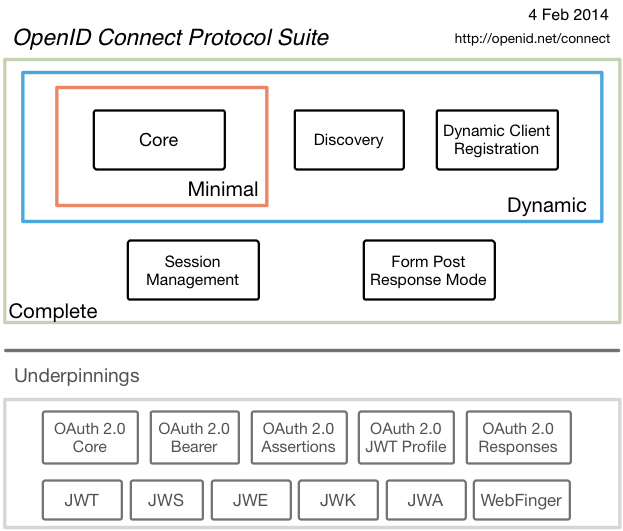
\includegraphics[width=0.7\textwidth]{figures/OpenIDC-map.png}
    \caption[OpenID Connect protocol suite]{OpenID Connect protocol suite\\\hspace{\textwidth}Source:\hspace{0.2cm}\url{https://openid.net/connect/}}
    \label{fig:oidc}
\end{figure}

Previously, the concepts of \textbf{federated identity} and \textbf{delegated authority} have been introduced and it has been mentioned that they are actually the same underlying concept. In one delegated authority scenario, the User delegates authority for a Client application to access some protected resource on their behalf, say, access to their Facebook friend list. However, this protected resource could be anything. It could even be their profile information as stored by Facebook. Delegating access to this resource gives the Client application the means of verifying the end-user's identity without ever seeing their credentials. As an example, it is interesting how this is accomplished with OpenID Connect using a familiar \oauth\ workflow. What follows is a modified version of the AuthZ Code Grant flow that we explored previously:

\begin{itemize}
    \item[1.] The Client application initiates the authorization request using the AuthZ Code Grant flow. However, in this authorization request, a subset of the following OpenID Connect scopes is requested:
    \item[] \begin{itemize}
        \item \texttt{openid}: REQUIRED. It means that the Client is making an OIDC request
        \item \texttt{profile}: OPTIONAL. This requests access to the User's
    profile information
        \item \texttt{email}: OPTIONAL. This requests access to the User's e-mail address
        \item \texttt{address}: OPTIONAL. This requests access to the User's  address information
        \item \texttt{phone}: OPTIONAL. This requests access to the User's phone number
    \end{itemize}
    
    \item[2.] Here the server must validate the parameters. In particular, OIDC defines more OPTIONAL parameters (e.g. \texttt{nonce}, \texttt{prompt}, and so on) that are essential for managing the authentication (e.g. rather than the authentication itself, whether the User is already authenticated or not). After that the server validates the parameters, if it is a valid request for login, the User is presented with the same User consent screen that we are familiar with, with the difference that it MAY be specified that the User authorizes the relying party (Client) to authenticate it. If it accepts, it will be redirected back to the Client application via the redirection endpoint, passing along with it the corresponding authorization code (as \oauth\ requires).
    \item[3.] The Client application will take this authorization code and make a request to the service provider's token endpoint to exchange it for an Access Token. The server must know that the corresponding AuthZ code was issued from an OIDC authentication request and must check the client\_id correspondence of it. It builds up the \texttt{id\_token} that is a JWT which contains private claims about the authenticated User (\texttt{name}, \texttt{address} and so on) and other claims defined in Section 4.1 of the \rfc{7519} \cite{RFC7519} (such as \texttt{iss} that represents the issuer and \texttt{sub} that represents a unique identifier of the authenticated User).
    \item[4.] The response from this request will contain an Access Token (as the property \texttt{access\_token}). However, it will contain the additional token known as an \textit{ID token} (as the property \texttt{id\_token}). The Client MUST decrypt the token by using the specified cryptographic operations contained in the JOSE Header (Section 5 of \rfc{7519}), validate the JWT ID Token, and retrieve the claims about the User, the issuer and so on, in order to ensure the truthfulness of the message response. Finally, the User identity provided by the AuthZ Server using OIDC on top of \oauth\ is verified.
\end{itemize}


As it can be seen, this flow is very similar to the AuthZ Code Grant flow that has been discussed earlier, except now it is possible to verify the identity of the User by consuming the ID token built and signed by the AuthZ Server, something that was not possible to do with \oauth\ alone. It is an elegant solution to provide a full end-to-end authentication and authorization framework.
% ------ END SECTION 3.2.4 ------
% ------ END SECTION 3.2 ------
% ------ END SECTION 3 ------

% ------ SECTION 4 ------
\section{Residual risks}
In this last section some important best practices are presented, along with a deep analysis of the common attacks on \oauth. All the risks linked to the protocol are described in Section 10 of the \rfc{6749} \cite{RFC6749}.

Security should always be a top priority. The security process must be combined with the implementation in order to avoid holes and expose the system to dangerous consequences.
Of all the unfortunate risks, the most treacherous ones are:

\begin{itemize}
    \item User impersonation
    \item Client impersonation
    \item Unauthorized access or permission granted
    \item Unauthorized access to data and/or resources
\end{itemize}

That is why the Client implementation must follows design best practises in order to avoid any risk and the programmer must be aware of the possible attacks.

% ------ SECTION 4.1 ------
\subsection{Best practices}
Since it is obvious that there is no way of zeroing the attack vectors available, the best choice is to minimise this vectors. In this section is presented a non-complete list of the best practices to follow when implementing an \oauth\ solution: 

\begin{itemize}
    \item \textit{Use the AuthZ Code Grant flow}. Since this grant type involves a trusted Client (\ie\ a Client that is capable of storing and transmitting securely private information), it is by far the most secure flow. The choice of not using this grant type is only acceptable for particular cases, where there is no way of having a back-end server or for the previously discussed reasons.
    \item \textit{Use TLS}. \oauth\ involves multiple endpoints for redirections and for other APIs. Even if it might seem an obvious best practice, not using TLS will break every other possible security choice, since all the important information and the parameters like the Access Token will be available for literally everyone during the transmission through the network.
    \item \textit{Use the Refresh Token}. As already mentioned in the previous sections, a Client that implements the AuthZ Code Grant flow SHOULD implements the Refresh Token flow. From a security perspective, the Refresh Token flow does not require the User, reducing its interactions and avoiding the frequent typing of username and password of its account on the AuthZ Server. Furthermore, the Refresh Token flow is much more resource-aware, since it exchanges only two messages.
    \item \textit{Use native browsers}. \label{native} During a native application implementation it can be chosen to use an embedded browser or open the native browser (in order to start a new flow). Even if the embedded browser provides a better user-experience, the best practice is not to use them. As explained in Section \ref{phishing}, the Phishing attack can stole the credentials by cheating the User. The embedded browser has much less information regarding the website (like the validity of the used certificate) with respect to the native browser. That is why native browsers must be preferred: they help the User to avoid this kind of attacks.
    \item \textit{Do not use third-party scripts in the redirection endpoint}. As stated in \cite{mastering}, "The redirection endpoint has to contain scripts only to remove the credentials before redirecting the agent to another page.". This is true because of the security capabilities of the untrusted Client in the Implicit Grant flow. More in details, when the User-agent redirects to the defined endpoint available on the Hosted Resource, the returned script is runned automatically. All of this in done in order to avoid the unwanted execution of third-party scripts that could leak or delay the Access Token extraction.
    \item \textit{Rotate the Client credentials}. \label{rotate} This is a well know best practice. Just as it has to be done with the passwords, rotating the credentials can limit in time the illegal use of leaked credentials. For example, they can be changed at each application release.
    \item \textit{Request minimal scopes}. As it was already described, the scopes are permissions that the Client requests on behalf of the User. It is important to take only what is needed, since during the application cycle and versioning some functionalities might change and some scopes are not required anymore, but still implicitly requested.
    \item \textit{When using the Implicit Grant flow, request read-only permissions}. As it has been discussed previously, Clients that utilise the Implicit Grant flow are untrusted Clients. This meas that the Access Token is not securely stored and the risks are higher. In order to minimise the consequences of an Access Token leak, the best choice is to request only read-only permissions.
    \item \textit{Credentials and tokens out of reach of Users}. If a User can see them, an attacker can see them. The Client credentials and the tokens are sensitive properties. The only way of keeping all as secure as possible it to have a trusted back-end server, capable of storing and transmitting these properties securely.
\end{itemize}
% ------ END SECTION 4.1 ------

% ------ SECTION 4.2 ------
\subsection{Common attacks analysis}
After the section dedicated to some security best practices used to keep the application safe, it is now time to take a look at some common attacks against \oauth\ Clients. For each attack, it will also be examined a mitigation technique that should be used in order to avoid it.

% ------ SECTION 4.2.1 ------
\subsubsection{Cross-site request forgery}
\label{csrf}
CSRF is a powerful attack that involves deceiving the Users by following a link that performs some bad actions on a trusted site (\eg\ a bank website). This attack exploits a pre-existing session with that site in order to provisionally gain access to the trusted site. The following example is taken from \cite{mastering}:

\begin{itemize}
    \item[] \textit{For instance, imagine a user has just logged into their bank in their favorite web browser. Now, in another tab, they open an e-mail from a malicious user with a link that says "See cats here!" which leads to \url{http://www.catloversheaven.com/}. This site is owned by the attacker and, while the user is browsing cute cat pictures, in the background, the website silently makes a call to \url{https://www.bank.com/transfer?to=37325283\&amount=1000}. Since the user already has a valid session with their bank, this request will be seen as valid. And so, while the user is enjoying the attacker-owned cat website, they have also unwittingly transferred \$1,000 out of their account and into the attacker's account.}
\end{itemize}


How is this relevant to an \oauth\ Client? 
Reminding the discussed flows, it is possible to add another party (namely, the attacker). In this scenario (\myfig{\ref{fig:csrf}}), the attacker sends an AuthZ Code (malicious, by using the victim open session) directly to the Client redirect URI. The Client can't verify the AuthZ Code and it uses the malicious AuthZ Code to request a malicious Access Token. As the Access Token is owned by the attacker, the attacker itself could gain access to the User protected resources.
This happens because the Client has no way of verifying that the Access Token is a result of a valid request.

\begin{figure}[ht]
    \centering
    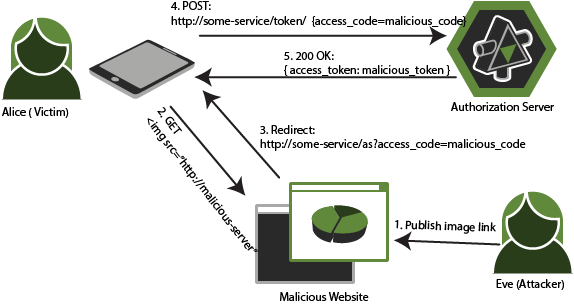
\includegraphics[width=0.9\textwidth]{figures/csrf.png}
    \caption[CSRF on \oauth]{CSRF on \oauth.\\\hspace{\textwidth}Source:\hspace{0.2cm}\url{https://stackoverflow.com/a/42520213}}
    \label{fig:csrf}
\end{figure}

To mitigate this attack, the Client must use the \texttt{state} parameter: an unguessable value generated by the Client during its requests and returned by the AuthZ Server during the responses. The Client must only accepts requests that contains the same parameter of its requests, discarding other malicious messages.

If a \texttt{state} parameter value is passed to a service provider, the \oauth\ protocol specifies that it MUST be returned back to the Client.
% ------ END SECTION 4.2.1 ------

% ------ SECTION 4.2.2 ------
\subsubsection{Phishing}
\label{phishing}
The Phishing attack aims at cheating the User by using a website or an application that looks very similar to the original one. In this scenario, the malicious website requests some personal information to the User, that is unaware of the risk and provides secret information like passwords or credit cards numbers.  

This attack applies to \oauth\ Client because, during the authorization request, the User is sent to the AuthZ Server by using the User-agent in order to delegate authority, providing its credentials. It is important that during the implementation of the Client the security implications of the User interaction with the AuthZ Server must be taken into account. A good advice is to follow some best practices (see \ref{native}).

Native browsers have some clear indicators about a site validity, like the lock icon when HTTPS is enabled (\myfig{\ref{fig:ioslock}}). Instead, embedded browsers can hide these information for a better user-experience, helping the attackers in their affairs.

\begin{figure}[ht]
    \centering
    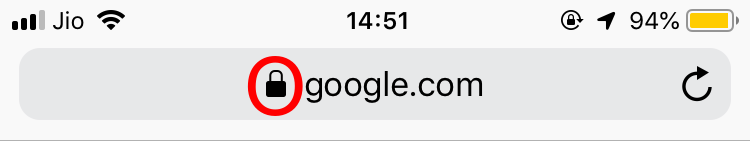
\includegraphics[width=0.9\textwidth]{figures/oie_toIlpPOFRMdK.png}
    \caption{Example of site validity on Safari for iOS}
    \label{fig:ioslock}
\end{figure}


% ------ END SECTION 4.2.2 ------

% ------ SECTION 4.2.3 ------
\subsubsection{Redirection URI manipulation}
During the authorization request, the Client passes the \texttt{redirect\_uri} param. This attack involves the injection of another \texttt{redirect\_uri} that could possibly redirect to a malicious server in order to stole secrets and Access Token. The following example is taken from \cite{mastering}:

\begin{itemize}
    \item[] \textit{For example, consider the scenario where the application GoodApp allows users to create a homepage on their domain. The user Eve may have a homepage that she controls at \url{www.goodapp.com/users/eve}. If the service provider that you are interacting with allows you to register wildcard redirect URIs, like \url{www.goodapp.com/*}, or doesn't require you to register your redirect URIs at all, then an attacker, such as Eve, would be able to use this homepage to her advantage. What Eve could do is set up a fake link to log into your application, or even a counterfeit application entirely. When a user clicks on this link, they will be directed to the authorization endpoint of the service provider just as would be done from the real application. However, instead of passing the proper redirect URI, say \url{www.goodapp.com/callback}, this link passes her own malicious redirect URI which just happens to be her profile page, \url{www.goodapp.com/users/eve}. On this page, she can then intercept any authorization codes and access tokens, and proceed to impersonate your users and access their protected resources.}
\end{itemize}

\begin{figure}[ht]
    \centering
    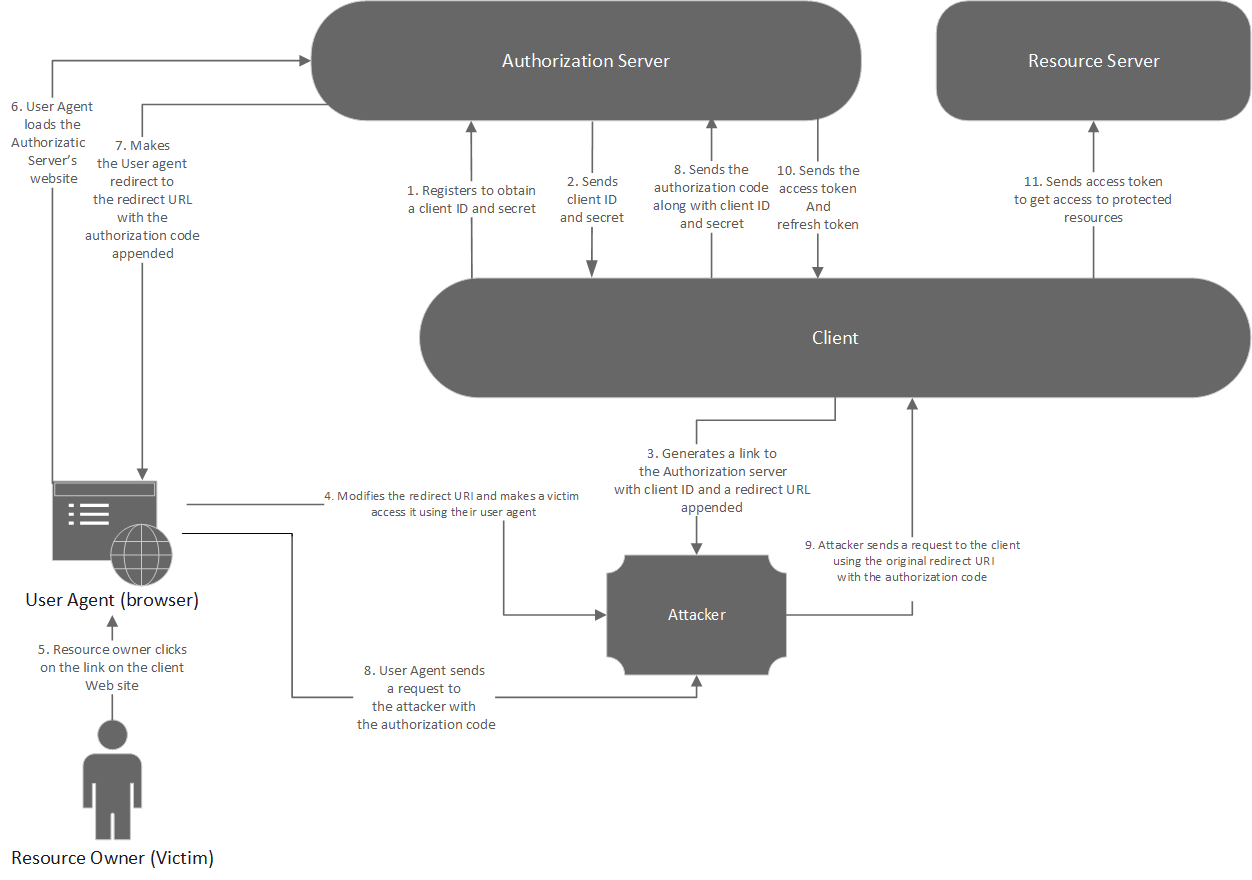
\includegraphics[width=0.9\textwidth]{figures/authCodeURIAttack.png}
    \caption[Redirection URI manipulation's typical flow]{Redirection URI manipulation's typical flow.\\Source:\hspace{0.2cm}\url{https://www.thearmchaircritic.org}}
    \label{fig:reduri}
\end{figure}


The only mitigation to this attack is the registration of the redirect URIs (\ie\ the authorized URIs must be known by the AuthZ Server) so that, if not allowed, the redirection will not take place. An example of a Redirection URI manipulation attack is shown in \myfig{\ref{fig:reduri}}.
% ------ END SECTION 4.2.3 ------

% ------ SECTION 4.2.4 ------
\subsubsection{Client and User impersonation}
Impersonation of Clients or Users is a well known and common attack.

"In Client impersonation, an attacker masquerades as the client application in order to gain access to the user's protected resources" \cite{mastering}. The Client credentials can be stolen by an attacker and used to impersonate the Client. A good practice in this scenario is the rotation the Client credentials (\ref{rotate}).

"In user impersonation, an attacker masquerade as the end user" \cite{mastering}. If the attacker accesses the issued Access Token, it could make requests to the Resource Server on behalf of the User.

In both the types of impersonation, the most effective mitigation technique is to hide everything (code, tokens, credentials) from the end User.

% ------ END SECTION 4.2.4 ------
% ------ END SECTION 4.2 ------
% ------ END SECTION 4 ------

% ------ SECTION 5 ------
\section{AuthZ Code Grant design}
In order to explain the \oauth\ protocol from a practical point of view, they have been designed and implemented two distributed application examples that uses the AuthZ Code Grant flow. 

The first implementation (henceforth referred as \textit{oauth-hw-security}) aims at explaining how to build a flow by using the proprietary Google/Facebook AuthZ Server and Resource Server, while the second one (henceforth referred as \textit{oauth-hw-security-custom}) aims at explaining how to build a flow by using custom AuthZ Server and Resource Server built from scratch.

The oauth-hw-security distributed application consists of two modules:

\begin{itemize}
    \item \textit{hw-server}: A Spring Boot implementation of the \oauth\ Client.
    \item \textit{hw-client}: A simple React application that consumes the APIs provided by the hw-server module.
\end{itemize}

As mentioned in Section \ref{authcg}, the Client is often a web-server that provides the web pages directly to the User, but this is not a constraint (according to the specification). In fact, the Client can only implement HTTP APIs so that they are consumed by web-applications or even native mobile applications and desktop applications. Thus, the hw-client module is not strictly necessary, but it is an example on how to correctly use the provided APIs.
The hw-server exposes the following APIs to the hw-client:

\begin{itemize}
    \item \textcolor{blue}{\texttt{\small http://localhost:8080/oauth2/authorize/<provider>?redirect\_uri=<redirect\_uri>}}\\
    This endpoint accepts only HTTP GET and "tells" to the Client to start an AuthZ Code Grant flow with \texttt{<provider>} (that can be "google" or "facebook") and, when finished, to redirect back to the hw-client on the \texttt{redirect\_uri}. When the Client finishes, it saves the User information into a database and calls the \texttt{redirect\_uri}, passing a local token to the hw-client.
    
    \item \textcolor{blue}{\texttt{\small http://localhost:8080/user/me}}\\
    This endpoint accepts only HTTP GET with the local token in the \texttt{Authorization} header. If the local token is valid, it returns a JSON with all the information of the User retrieved from the database, rendered into the Profile page of the \textit{hw-client}.
\end{itemize}

In this distributed application, the hw-server acts like a server that is interested in the User's base information in order to register the User and create an account of the User in the database (\ie\ the "Sign up with" link that some websites have). Moreover, the hw-server implements a simple email/password registration and login (to complete the solution functionalities). Finally, the local token is a simple token used for accessing these information in the database and it is not related to \oauth.

The oauth-hw-security-custom distributed application consists of three modules:

\begin{itemize}
    \item \textit{oauth2-client}: A Jakarta EE implementation of the \oauth\ Client (with respect to the oauth-hw-security solution, it is a web-server too, that presents some basic pages like the home-page on the User-agent to the User).
    \item \textit{oauth2-authorization-server}: A Jakarta EE implementation of the \oauth\ AuthZ Server.
    \item \textit{oauth2-resource-server}: A Jakarta EE implementation of the \oauth\ Resource Server.
\end{itemize}

For educational purposes, the home-page of the oauth2-client shows all the configuration info (Client registration info and, when available, the Access Token and Refresh Token). Furthermore, from this page the User can:
\begin{itemize}
    \item Start the AuthZ Code Grant flow by clicking on the "Get Access Token" link.
    \item Start the Refresh Token flow by clicking on the "Refresh Token (original scope)" link.
    \item Force the Refresh Token flow by clicking on the "Refresh token (scope:resource.read)" or "Refresh token (scope:resource.write)" link.
    \item Request to write the protected resource to the oauth2-resource-server by clicking on the "Write Protected Resource".
    \item Request to read the protected resource to the oauth2-resource-server by clicking on the "Read Protected Resource".
\end{itemize}

In addition, the oauth2-authorization-server module has two web pages used to perform the User login and the User consent, that are presented to the User when a new AuthZ Code Grant flow is started.
More details concerning the messages exchanged and the implementation are presented in the Programmer Manual (\ref{progman}).
% ------ END SECTION 5 ------

% ------ SECTION A ------
\appendix
\section{User manual}
This appendix explains how to correctly install and run the two implementations of the \oauth\ AuthZ Code Grant flow.

% ------ SECTION A.1 ------
\subsection{Software dependencies}
\label{appa}
Before installing and running the two implementations, there are some basic dependencies to install: \texttt{Docker} and \texttt{Docker-Compose}.

\label{ublin}
The Docker Documentation \cite{docker} explains how to correctly install Docker on Windows/Ubuntu/macOS.

\paragraph{Ubuntu Linux (16.04 - 18.04 - 20.04)} First, all previous versions must be removed. 

From the bash terminal:
  
\quad \texttt{\$ sudo apt-get remove docker docker-engine docker.io containerd runc}

Update and install packages to install dependencies over HTTPS:

\quad \texttt{\$ sudo apt-get update}

\quad \texttt{\$ sudo apt-get install apt-transport-https ca-certificates curl \textbackslash}

\hspace{1cm} \texttt{gnupg-agent software-properties-common}

Add Docker's official GPG key:

\quad \texttt{\$ curl -fsSL https://download.docker.com/linux/ubuntu/gpg | sudo apt-key add -}

Set-up the \textbf{stable} repository (change the \texttt{arch} parameter according to the architecture):

\quad \texttt{\$ sudo add-apt-repository \textbackslash}

\hspace{1cm} \texttt{"deb [arch=amd64] https://download.docker.com/linux/ubuntu \textbackslash}

\hspace{1cm} \texttt{\$(lsb\_release -cs) stable"}

Install Docker:

\quad \texttt{\$ sudo apt-get update}
  
\quad \texttt{\$ sudo apt-get install docker-ce docker-ce-cli containerd.io}

Add the current User to the \texttt{docker} group:
  
\quad \texttt{\$ sudo groupadd docker}
  
\quad \texttt{\$ sudo usermod -aG docker \$USER}

For different Linux distros or architectures, the Official Docs\footnote{\url{https://docs.docker.com/engine/install/}} is available.

\paragraph{Windows 10 Pro/Enterprise ($\geq Build 15063$)} The steps to follows are pretty straightforward:

\begin{itemize}
    \item[1.] Download Docker Desktop from the download page\footnote{\url{https://hub.docker.com/editions/community/docker-ce-desktop-windows/}}.
    \item[2.] Ensures that Hyper-V is enabled\footnote{\url{https://docs.microsoft.com/en-us/virtualization/hyper-v-on-windows/quick-start/enable-hyper-v}}.
    \item[3.] Double-click on the installer downloaded.
    \item[4.] Follow the standard installation procedure.
\end{itemize}

\paragraph{macOS ($\geq 10.13$)} Similarly to Windows:

\begin{itemize}
    \item[1.] Download Docker Desktop from the download page\footnote{\url{https://hub.docker.com/editions/community/docker-ce-desktop-mac/}}.
    \item[2.] Double-click on the \texttt{.img} downloaded.
    \item[3.] Drag the application in the Application folder.
\end{itemize}

For Windows and macOS systems, \texttt{docker-compose} is included in the Docker Desktop installation. On Ubuntu Linux, the steps follow.

Install PIP:

\quad \texttt{\$ sudo apt update}
  
\quad \texttt{\$ sudo apt install python3-pip}

Upgrade PIP:

\quad \texttt{\$ sudo pip3 install -U pip}

Install docker-compose:
  
\quad \texttt{\$ sudo pip3 install docker-compose}
% ------ END SECTION A.1 ------

% ------ SECTION A.2 ------
\subsection{Installation and use}
Once that \texttt{docker} and \texttt{docker-compose} are installed, the demos installation and use is not OS-dependent. Indeed, Docker Desktop (Windows/macOS) needs to be started as application first.

% ------ SECTION A.2.1 ------
\subsubsection{oauth-hw-security}
In order to install and run the implementation example that interacts with Google/Facebook, the file \textbf{docker-compose.yaml}\footnote{\url{https://github.com/nopesir/oauth-hw-security/releases}} is available in the resources as well as on GitHub as shown in \myfig{\ref{fig:rel1}} (there are other files, but we only need the \texttt{.yaml} file).

\begin{figure}[ht]
    \centering
    \fbox{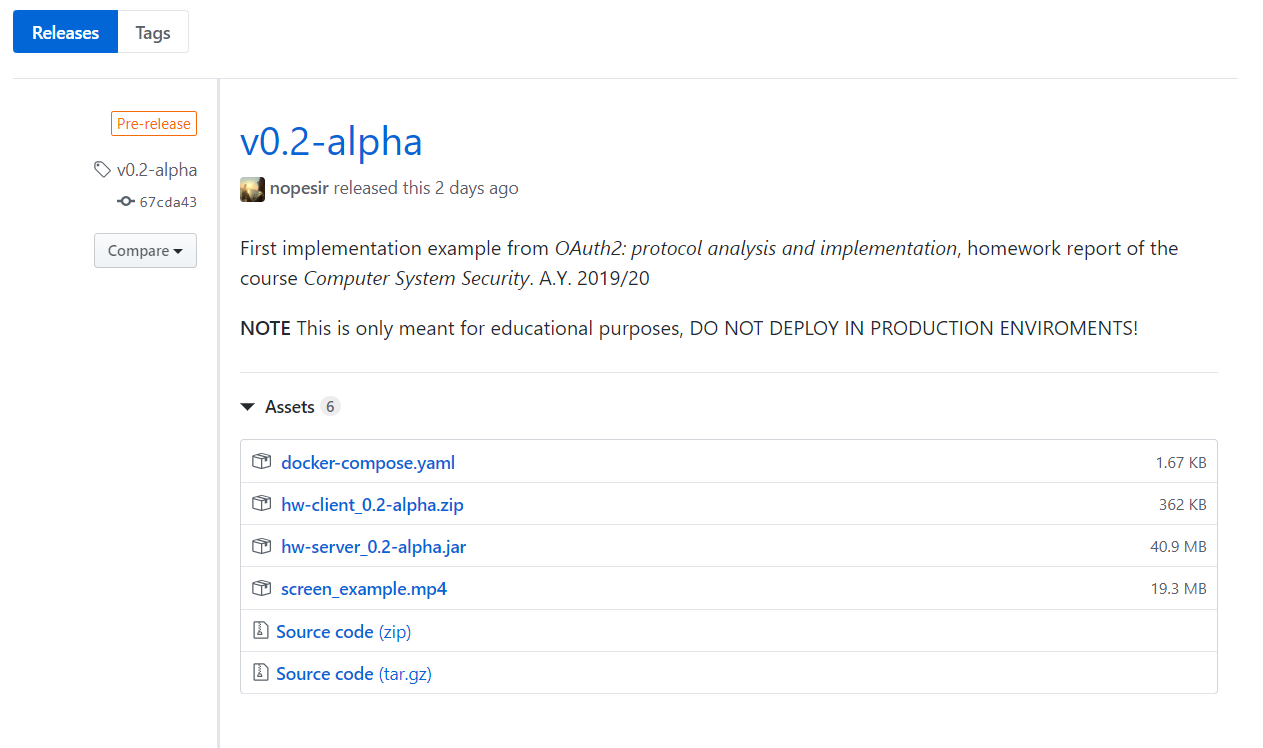
\includegraphics[width=0.9\textwidth]{figures/release1.png}}
    \caption{GitHub Releases page: where to download the \texttt{docker-compose.yaml} file}
    \label{fig:rel1}
\end{figure}

Then, in the same folder where \textbf{docker-compose.yaml} is, from the terminal:

\quad \texttt{\$ docker-compose up}

If all the dependencies are correctly installed and the docker daemon is running, \texttt{docker-compose} will automatically pull the containers, create the network namespace and start everything. The first run needs some time to download, but the next ones will use the downloaded data and will boot up the containers in a few seconds. The application now is running. From the browser, visit \url{http://localhost:9090} and the homepage will be displayed (\myfig{\ref{fig:home1}}).

\begin{figure}[ht]
    \centering
    \fbox{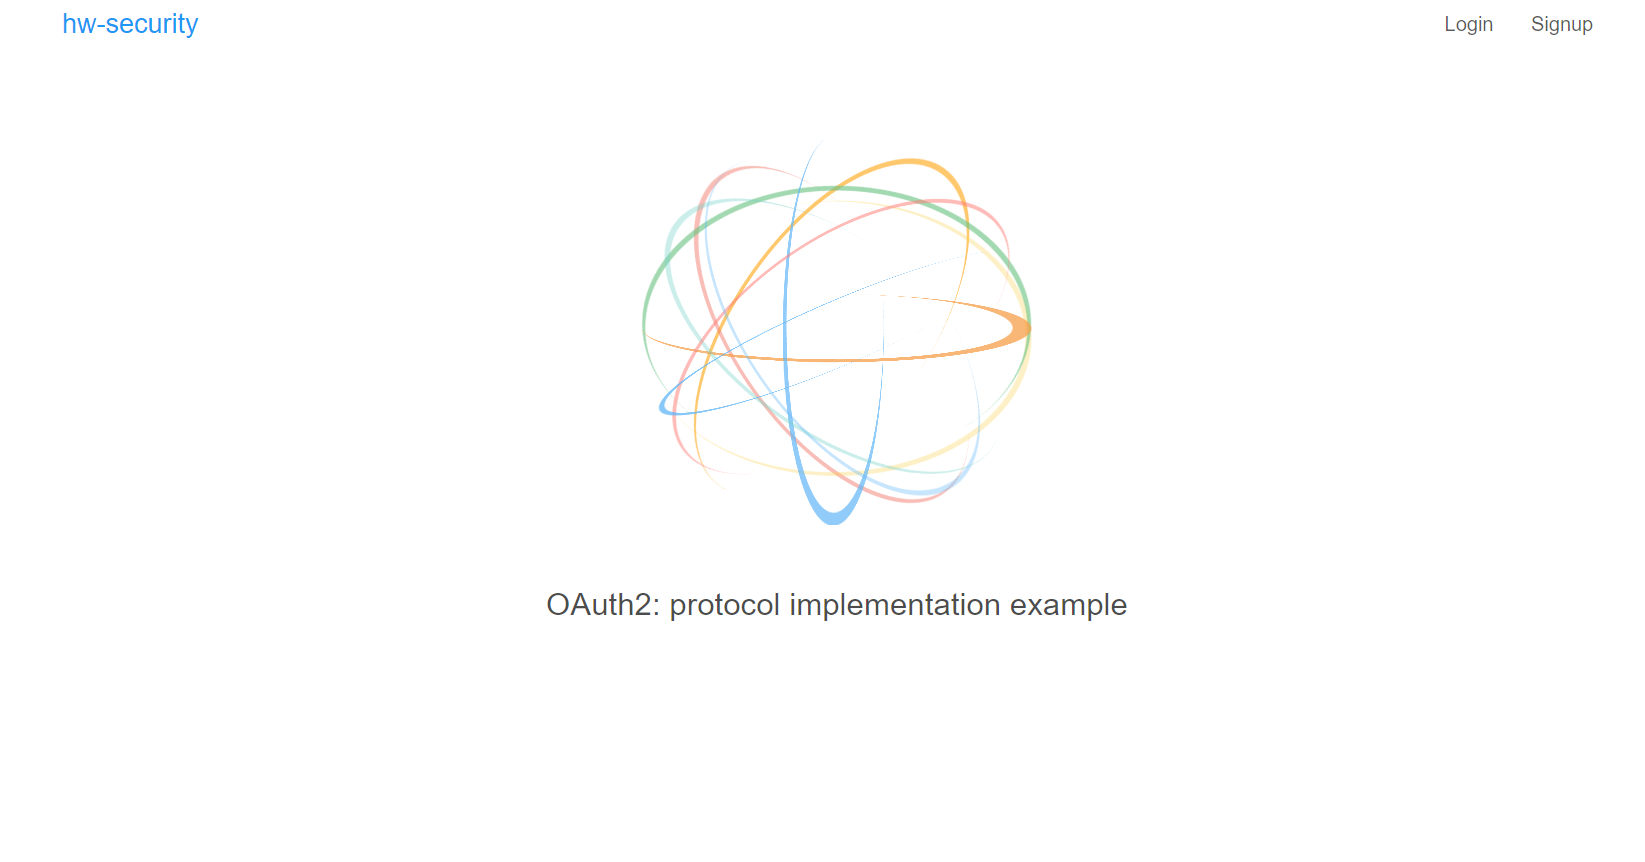
\includegraphics[width=0.9\textwidth]{figures/screen1.png}}
    \caption{The homepage of the first implementation example}
    \label{fig:home1}
\end{figure}

To stop the application and safely detach all the resources, \texttt{Crtl+C} command on the terminal and finally a:

\quad \texttt{\$ docker-compose down}

The full screen video captioning of the example is available in the resources and in the Assets of the releases page\footnote{\scriptsize{\url{https://github.com/nopesir/oauth-hw-security/releases/download/v0.2-alpha/hw-security-screen.mp4}}}. 

\paragraph{Troubleshooting}
\begin{itemize}
    \item Ensure to have ports \texttt{9090/tcp}, \texttt{8080/tcp} and \texttt{3306/tcp} available.
    \item Facebook login could give an error: Facebook App in test mode are accessible with \oauth\ only by the developer Facebook account\footnote{\url{https://developers.facebook.com/docs/apps/managing-development-cycle/\#step1}}, thus some test users must be added to the Facebook Developer's page. Use Google instead.
    \item Ensure to have at least 8GB of RAM on the machine.
    \item (Windows/macOS) Ensure that the Docker Desktop program is started.
    \item (Ubuntu Linux) Ensure that the Docker daemon is running.
\end{itemize}
% ------ END SECTION A.2.1 ------

% ------ SECTION A.2.2 ------
\subsubsection{oauth-hw-security-custom}
In order to install and run the second example, the steps are almost the same as the previous subsection. The new \textbf{docker-compose.yaml} is available on the releases page\footnote{\url{https://github.com/nopesir/oauth-hw-security-custom/releases}} or in the resources (remove the previous \texttt{.yaml} file or choose another folder).

Then, in the same folder where \textbf{docker-compose.yaml} is, from the terminal:

\quad \texttt{\$ docker-compose up}

If all the dependencies are correctly installed and the docker daemon is running, \texttt{docker-compose} will automatically pull the containers, create the network namespace and start everything. 
The first run needs some time to download, but the next ones will use the downloaded data and will boot up the containers in seconds. The application now is running. From the browser, visit \url{http://localhost:9180} and the homepage will be displayed (\myfig{\ref{fig:home2}}).

\begin{figure}[ht]
    \centering
    \fbox{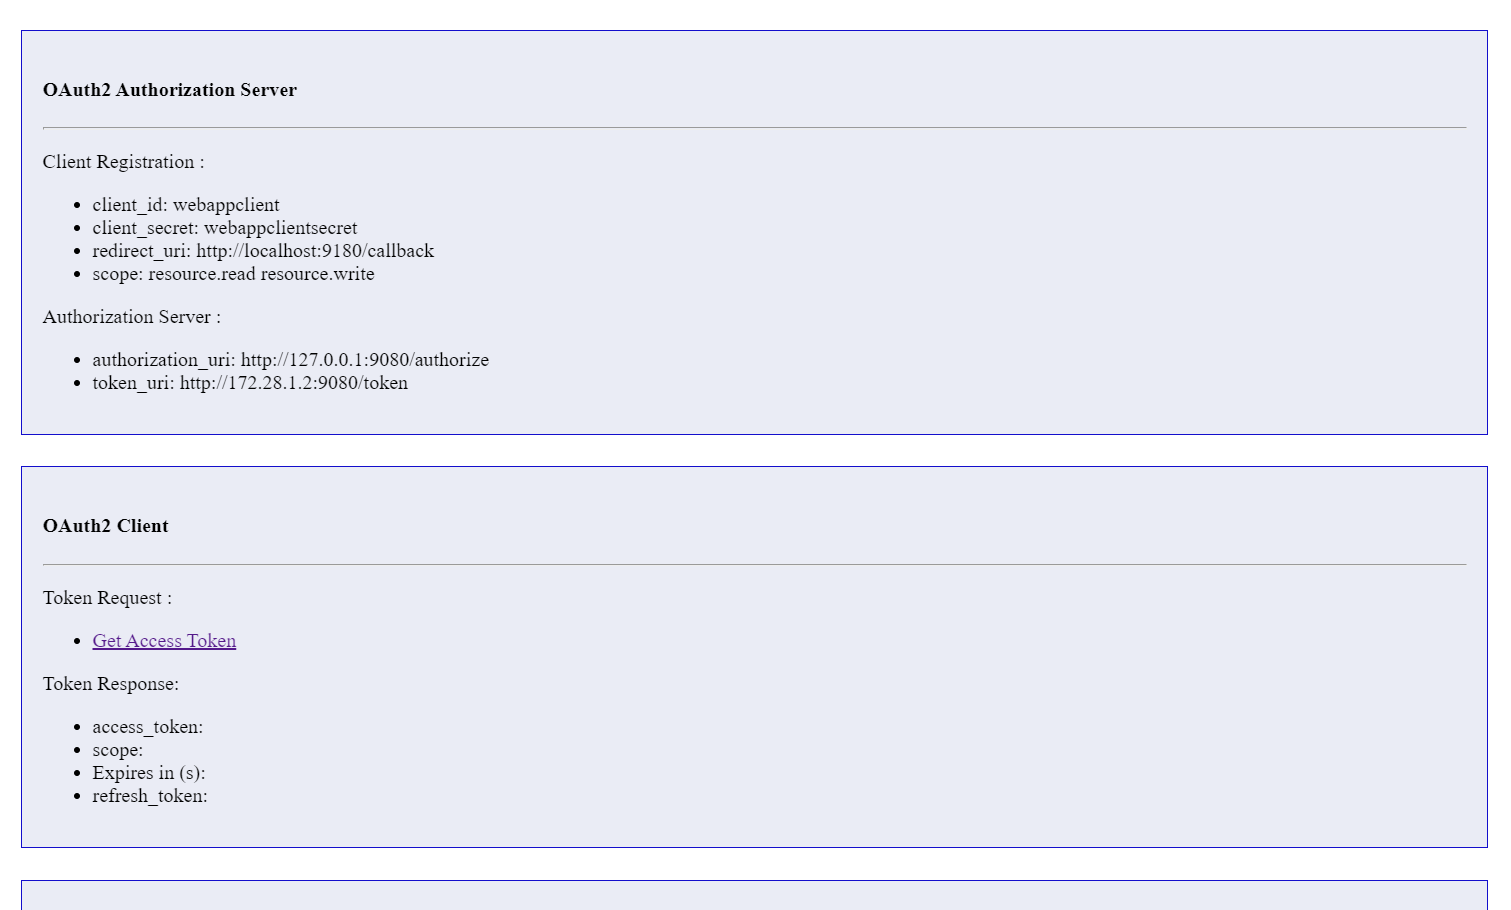
\includegraphics[width=0.9\textwidth]{figures/screen2.png}}
    \caption{The homepage of the second implementation example}
    \label{fig:home2}
\end{figure}

Since this is an educational example, all the information are in plain text in the homepage. The first thing to do is to retrieve the Access Token by clicking on the link. Then, a log-in is necessary. The only available credentials are:

\begin{itemize}
    \item Username: \textit{appuser}
    \item Password: \textit{appusersecret}
\end{itemize}

After the log-in, it is displayed a checkbox in order to select what authorizations will be delegated to the Client app. Select \texttt{resorce.read}, \texttt{resource.write} or both. 
Finally, the User will be redirected to the homepage with an Access Token. Now, it is time to request the resource using the two links at the end of the page. If the Client is authorized, it will print a simple message, otherwise a 403 HTTP error is displayed (Forbidden). In addiction, it is available the Refresh Token flow based on the authorized resources or a subset of them (e.g. if someone has the Access Token for both scopes, it can make the token refresh for only one too). To stop the application and safely detach all the resources, \texttt{Crtl+C} command on the terminal and finally:

\quad \texttt{\$ docker-compose down}

The full screen video captioning of the example is available in the Assets of the releases page\footnote{\scriptsize{\url{https://github.com/nopesir/oauth-hw-security-custom/releases/download/v0.5-alpha/hw-security-custom-screen.mp4}}} or in the resources.
% ------ END SECTION A.2.2 ------
% ------ END SECTION A.2 ------
% ------ END SECTION A ------

% ------ SECTION B ------
\section{Programmer manual}
\label{progman}
This appendix explains how the two implementations are designed. In particular, there is a first section about the frameworks and the libraries used, followed by the implementation itself (with code explanations, problems, resolutions, endpoints and messages exchanged in practice) for both the examples. Finally, the last section is devoted to the compilation and dockerization of the solutions.

% ------ SECTION B.1 ------
\subsection{Frameworks, libraries and environment}
For what concerns the second demo and the hw-server of the first demo, it has been used Apache Maven as build automation tool and the only requirement is Java JDK8 installed. Moreover, since Maven is integrated into the project (by using maven-wrapper), there is no need to install it on the machine.
For what concerns the hw-client in the first demo, React is the Javascript framework chosen. The programs \texttt{npm} and \texttt{node} must be installed on the machine (see \url{https://www.npmjs.com/get-npm} to get both of them). 
The code of the implementation examples is available on GitHub:

\begin{itemize}
    \item \textbf{ouath-hw-security}\footnote{\url{https://github.com/nopesir/oauth-hw-security}}
    \item \textbf{oauth-hw-security-custom}\footnote{\url{https://github.com/nopesir/oauth-hw-security-custom}}
\end{itemize}

Last but not least, both \textit{Docker} and \textit{Docker-Compose} must be installed too to dockerize the solutions. For instructions, see (\ref{appa}). In the following last subsections are analysed the design and implementation of the two solutions with messages exchanged and endpoints used. The "Playground" demo provided by OAuth.com in collaboration with Okta \cite{playgr} can be very helpful for the developer to understand the flows and the protocol from a practical point of view. 
% ------ END SECTION B.1 ------

% ------ SECTION B.2 ------
\subsection{Implementation: oauth-hw-security}
The hw-server is a Spring Boot application that uses \oauth\ by exploiting Spring Security in order to implement both social (Google/Facebook/GitHub) and email/password logins (with a MySQL database). On the other hand, the hw-client application is not strictly related to \oauth, but it is an example on how to use the information provided by the \oauth\ Spring Boot server to interact with an end-user (in this case, a React web application). Since the flow with some providers varies for what concerns payloads types and endpoints, of particular relevance are the official documentations from Facebook \cite{facebook} and Google \cite{google1, google2}. Furthermore, to implement the Spring Boot server, a good example can be found on the developer.okta.com's blog \cite{sprboot}. 

The implemented flow's main actor is the Spring Boot server, that acts as a \oauth\ Client. The objective of this implementation is to retrieve basic User information (name and email) from the Google account by using the AuthZ Code Grant flow. More in details, this is done through a React web-app that consumes the server's APIs. The first interaction takes place as follows (for more details on the messages exchanged, see \myfig{\ref{fig:google1}}):

\begin{figure}[ht]
    \centering
    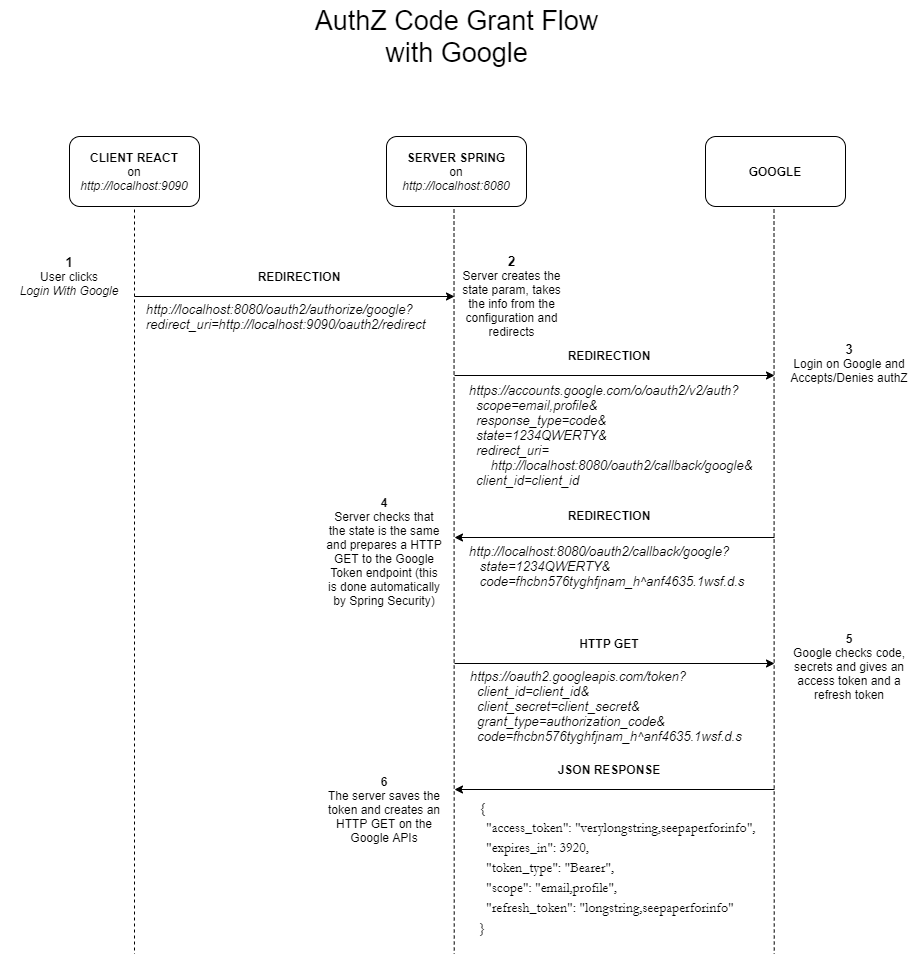
\includegraphics[width=0.85\textwidth]{figures/flow_google1.png}
    \caption{Implementation of the AuthZ Code Grant flow with Google. Part 1.}
    \label{fig:google1}
\end{figure}

\begin{enumerate}
    \item From the "Login" page, the User clicks on "Login With Google" and a first redirection starts on \url{http://localhost:8080/oauth2/authorize/google} with the requested parameters.
    \item The server creates the state parameter, takes the info from the configuration and redirects the User to the Google \oauth\ page (\url{https://accounts.google.com/o/oauth2/v2/auth}).
    \item Here the User logs in on Google and Accepts/Denies the AuthZ scopes. After the User acceptance, Google redirects it back on the server with the AuthZ Code.
    \item The server checks that the state is the same and prepares a HTTP GET to the Google Token endpoint (this is done automatically by Spring Security, no action is required by the User).
    \item Google checks code, secrets and gives a JWT Access Token and Refresh Token in a JSON object.
    \item The server saves the token.
\end{enumerate}

The second interaction starts in order to let the server populate the database by consuming the received token and giving a local token to the React web-app in order to let the app access the stored information in the database (\myfig{\ref{fig:google2}}):

\begin{figure}[ht]
    \centering
    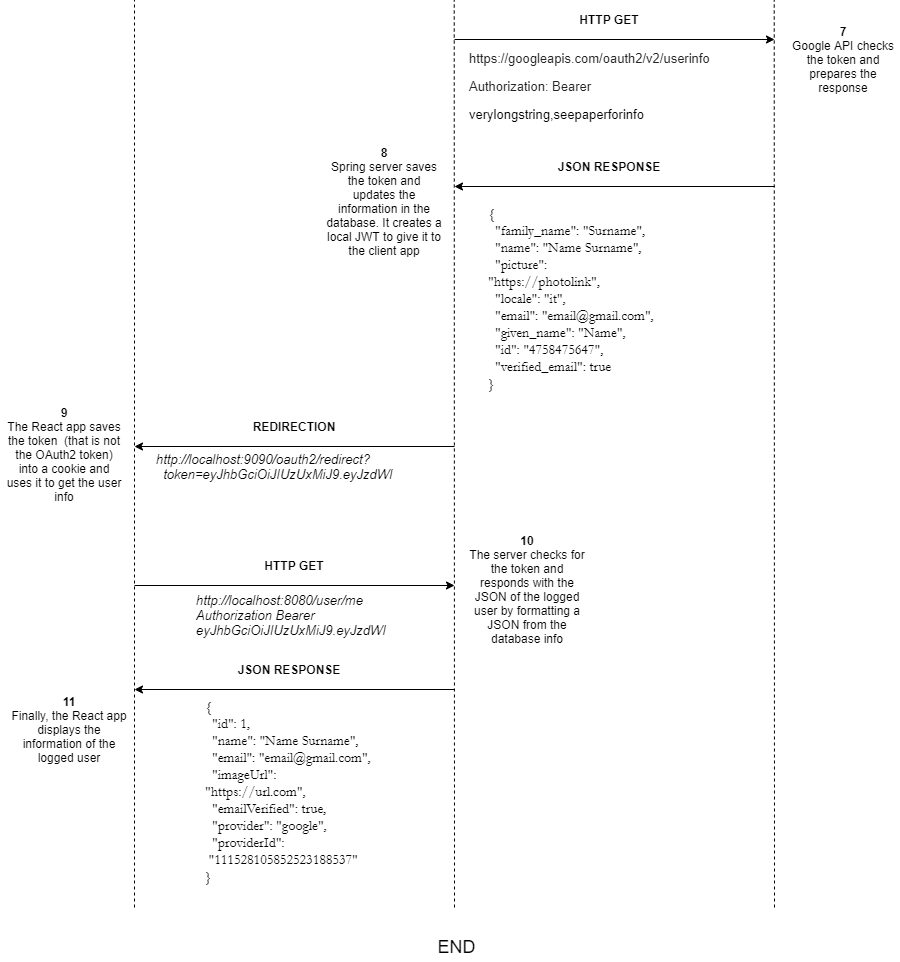
\includegraphics[width=0.85\textwidth]{figures/flow_google2.png}
    \caption{Implementation of the AuthZ Code Grant flow with Google. Part 2.}
    \label{fig:google2}
\end{figure}

\begin{enumerate}
    \item[7.] The server sends an HTTP GET to the Google endpoint \url{https://googleapis.com/oauth2/v2/userinfo} by inserting the \texttt{access\_token} in the authorization header. The Google API server checks the token and prepares the response as JSON.
    \item[8.] The Spring server saves the Access Token and updates the information in the database. It creates a local JWT token to give it to the Client app.
    \item[9.] The React app saves the token  (that is not the \oauth\ token) into a cookie and uses it to get the User info from the endpoint of the Spring server \url{http://localhost:8080/user/me} by attaching the local token into the authorization header.
    \item[10.] The server checks for the token and responds with the JSON of the logged User by formatting a JSON from the database info.
    \item[11.] Finally, the React app displays the information of the logged User.
\end{enumerate}

After this introduction on the general flow, in the following subsections is presented a detailed explanation of the implementation, divided into the two modules that compose the architecture.

% ------ SECTION B.2.1 ------
\subsubsection{hw-client}

As mentioned before, this application is pretty simple and it is only used as an interface between the \oauth\ Spring Boot back-end server and the User to display information. An alternative could be directly to implement into the Spring Boot back-end the web-server.

\begin{figure}[ht]
    \centering
    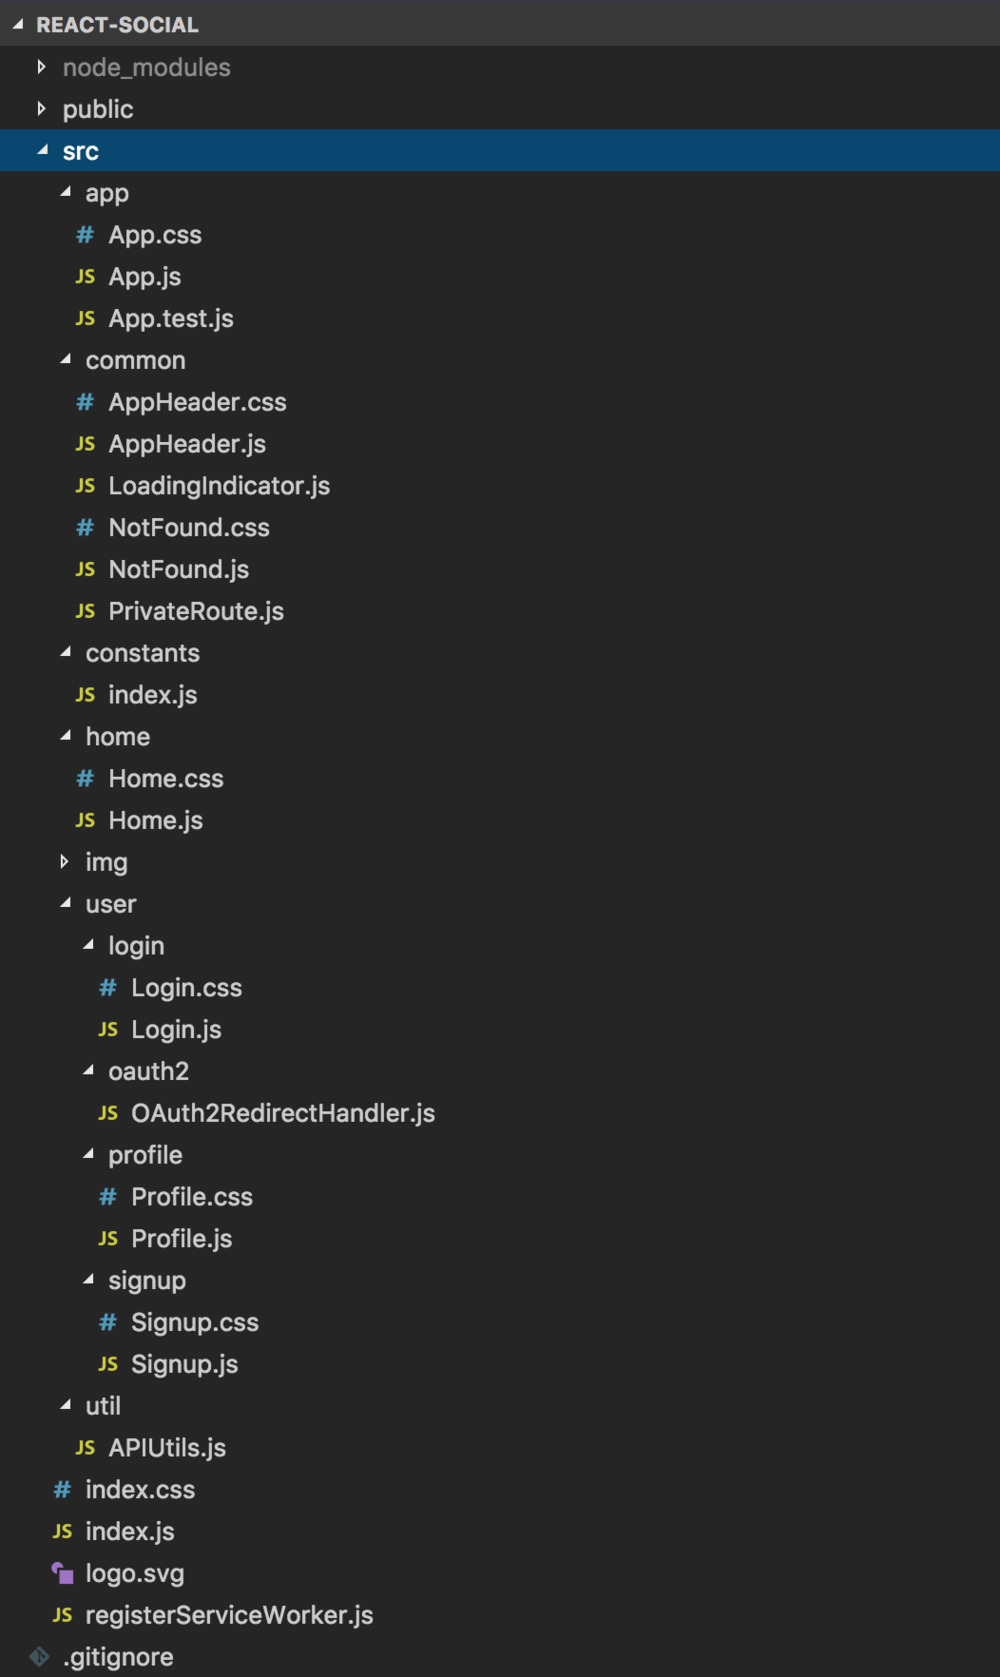
\includegraphics[width=0.30 \textwidth]{figures/dirreact.jpg}
    \caption{Final directory tree of the \texttt{react-social} app}
    \label{fig:dirtree}
\end{figure}

To create the base React application, simply type:

\quad \texttt{\$ npm install -g create-react-app}
  
\quad \texttt{\$ create-react-app react-social}

And then add the dependencies for routing and alerts:

\quad \texttt{\$ cd react-social}
  
\quad \texttt{\$ npm install react-router-dom react-s-alert --save}

That is the base React application to build on. We have to populate and organise the final directory structure to look like in \myfig{\ref{fig:dirtree}}.

The code is pretty self-explanatory, but there are some important aspects to consider. The first one is \textbf{index.js}, that is the entry-point of the application. It renders the App component in a document object model that has \texttt{root} as id and it is subsequently wrapped into a Router to enable hw-client routing. The second important aspect is \textbf{App.js}, located in \texttt{src/app}. It is the top-level element of the application and is responsible for the layout, the routes and manages the authentication by loading the details from the back-end of the current User, forwarding it to the child components. The \textbf{Login.js} file, located in \texttt{src/user/login}, is responsible for the \oauth\ login and the username/password login, while \textbf{OAuth2RedirectHandler.js} is the component called by the Spring Boot server when the User has completed the \oauth\ flow on it. In particular, once that the server flow is finished, the server saves all the information in a database and generates a local token. This component will receive a bearer token from the Spring Boot server (note that this token is not related to \oauth, it is a token generated by the Spring Boot server to manage the access to the database information) or an error otherwise.

Last but not least, the \textbf{index.js} located in \texttt{src/constants} contains information about the endpoints. The \texttt{\small API\_BASE\_URL} refers to the Spring Boot server base URL, that represents the API for the \textit{hw-client} app. The \texttt{\small OAUTH2\_REDIRECT\_URI} is the redirection URI where the \textbf{OAuth2RedirectHandler.js} is waiting to handle the response and the three \texttt{\small PROVIDER\_AUTH\_URL} are the Spring Boot server URLs called when the User clicks on one of the three \oauth\ login, passing as parameter a \texttt{redirect\_uri} to let the server know where to redirect the local token once that he has completed the AuthZ Code Grant flow. 

\begin{figure}[ht]
    \centering
    \fbox{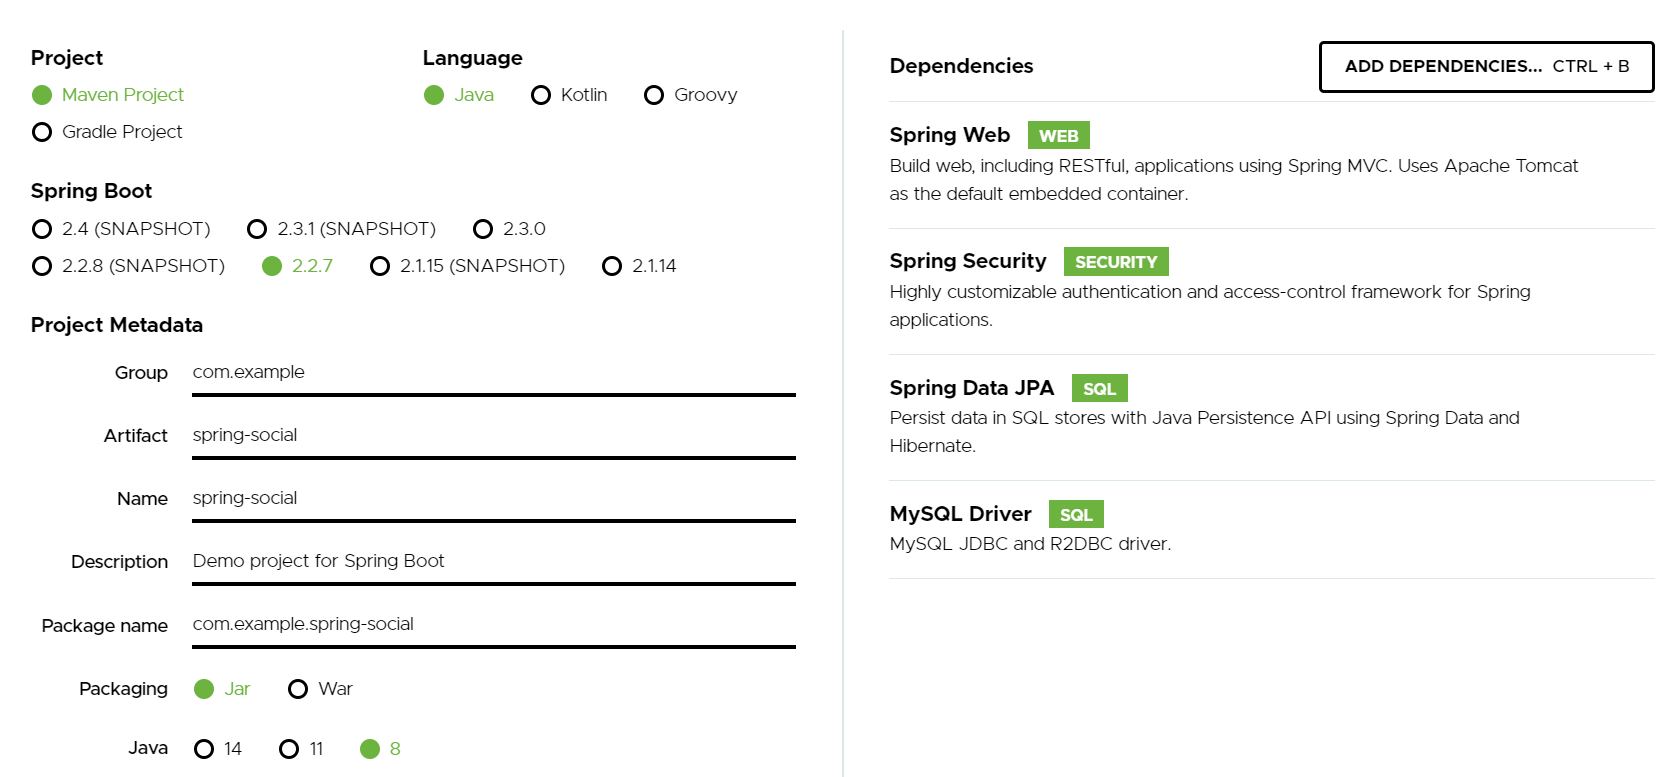
\includegraphics[width=16cm]{figures/spring.png}}
    \caption{Spring Boot base project selection}
    \label{fig:spring}
\end{figure}
% ------ END SECTION B.2.1 ------

% ------ SECTION B.2.2 ------
\subsubsection{Registration process}

\label{regprocess}
To enable the Spring Boot server to perform a social login with an \oauth\ provider, the first step is to create an application in the provider's developer console and obtain the \texttt{client\_id} and \texttt{client\_secret}. These two strings are used by the providers (Google, Facebook and so on) to identify our server application. Besides, there are some other parameters to consider:

\begin{itemize}
    \item \textit{Authorized redirect URIs}: After that the AuthZ Code Grant flow finishes, the provider needs this URI to understand where the User has to be redirected after the flow and what are the ones that are authorized by the developer.
    \item \textit{Scopes}: They represent \textbf{what} can be granted. Note that this is only meant to enable the possibility to give it, it is not automatically given to our server. The User will decide what scopes from the enabled scopes can be consumed by the Spring Boot server.
\end{itemize}

To create an app, simply start a new app in one of the following provider's page:

\begin{itemize}
    \item Google Project: \url{https://console.developers.google.com/}
    \item Facebook: \url{https://developers.facebook.com/apps}
    \item GitHub: \url{https://github.com/settings/apps}
\end{itemize}

More in details, for Google:

\begin{enumerate}
    \item Create a new project in the console.
    \item Go to \textit{APIs\&Services} $\,\to\,$ \textit{OAuth Consent Screen}. Select \textit{External} and then press \textit{Create}.
    \item Set an application name, and checks that the default scopes are present (\texttt{email}, \texttt{openid}, \texttt{profile}). Hit \textit{Save}.
    \item From the \textit{Credentials} page, \textit{CREATE CREDENTIALS} $\,\to\,$ \textit{OAuth Client ID}.
    \item Set as application type \textit{Web application} and in section \textit{Authorized redirect URIs} add an uri: \url{http://localhost:8080/oauth2/callback/google}. Hit \textit{Create}.
    \item Copy the \texttt{client\_id} and \texttt{client\_secret} and insert both of them into the \textbf{docker-compose-build.yaml} file (\texttt{client\_id\_g} and \texttt{client\_secret\_g}) before building it.
\end{enumerate}
% ------ END SECTION B.2.2 ------

% ------ SECTION B.2.3 ------
\subsubsection{hw-server}

\begin{figure}[ht]
    \centering
    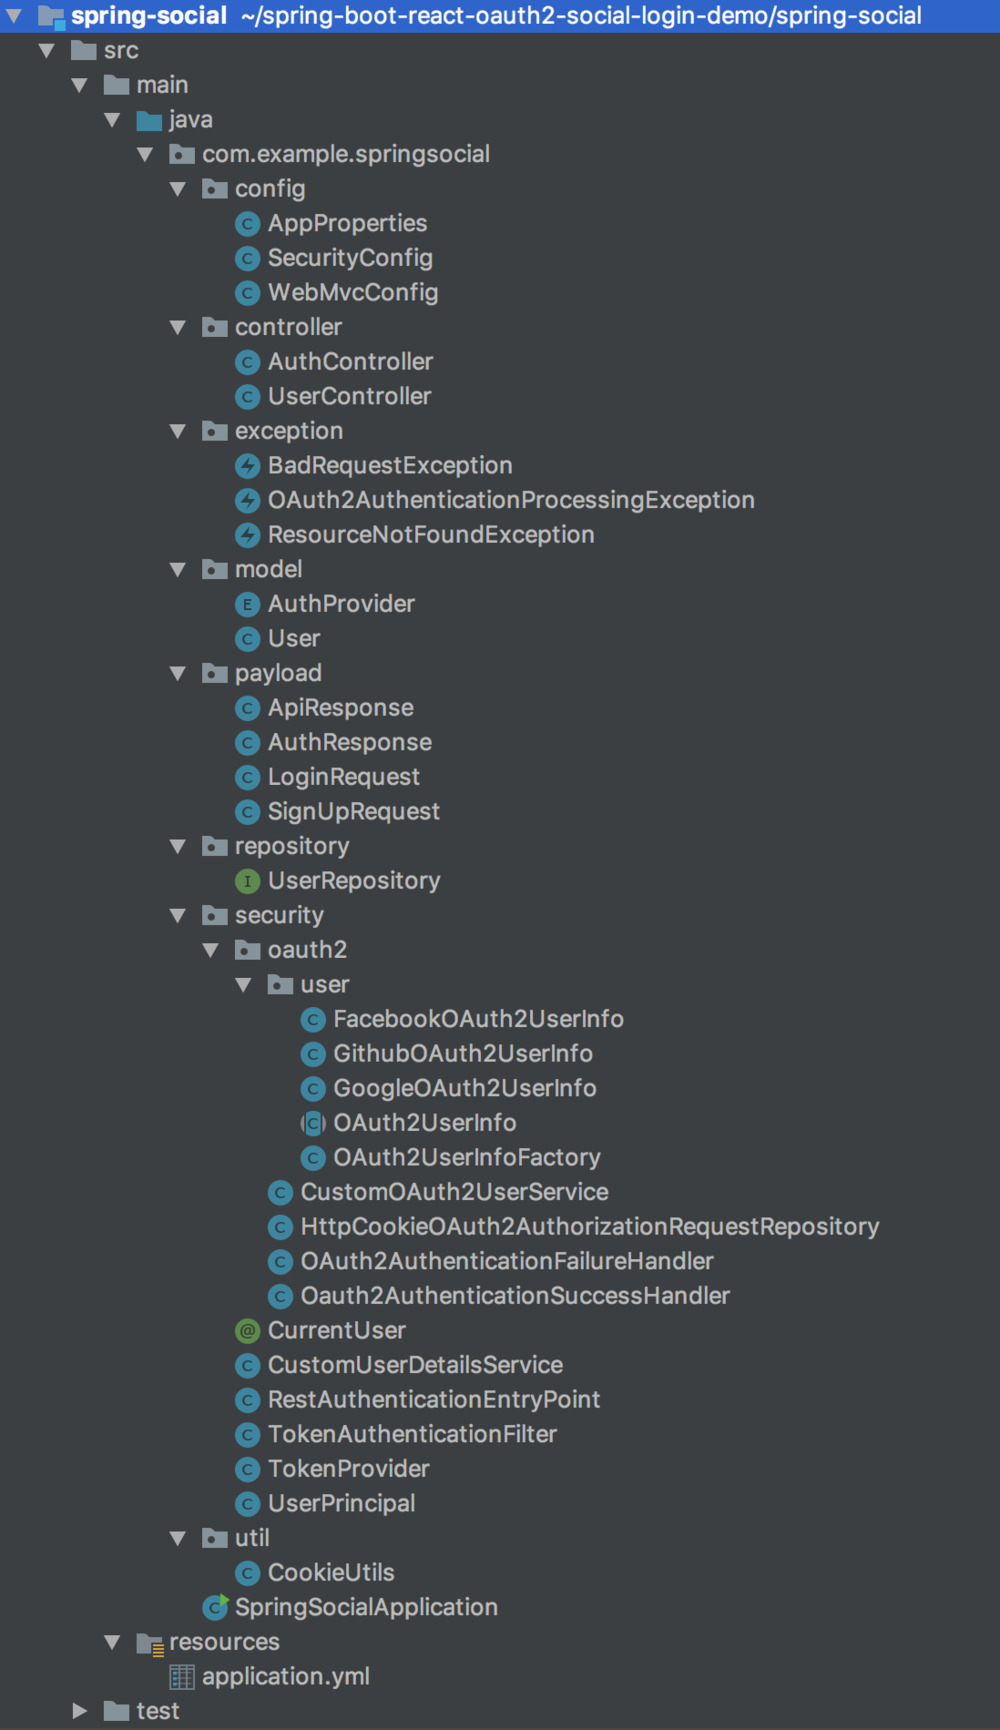
\includegraphics[width=0.3 \textwidth]{figures/springdir.jpg}
    \caption{Final directory tree of the Spring Boot hw-server}
    \label{fig:dirsocial}
\end{figure}

The server, as it has already mentioned, is a Spring Boot application. The base project can be automatically created using Spring Initializr\footnote{Start the project from \url{https://start.spring.io/}}. In particular, the selections are the ones in \myfig{\ref{fig:spring}}.

Then, the project folder has been modified to have the directory structure in \myfig{\ref{fig:dirsocial}}. Furthermore, two more dependencies must be added to the project (not available on Spring Initializr): \textit{\oauth\ Client} and \textit{JWT Library}. By opening the \texttt{pom.xml} file, thanks to Maven, simply add these lines into the \texttt{<dependencies></dependencies>} tags:

\begin{lstlisting}[language=XML, basicstyle=\ttfamily]
  <!-- OAuth2 Client -->
  <dependency>
    <groupId>org.springframework.security</groupId>
    <artifactId>spring-security-oauth2-client</artifactId>
  </dependency>

  <!-- JWT library -->
  <dependency>
    <groupId>io.jsonwebtoken</groupId>
    <artifactId>jjwt</artifactId>
    <version>0.5.1</version>
  </dependency>
\end{lstlisting}

Now that the Spring Boot app structure is ready, we are going to analyse every Java file and configuration file to understand how the functionalities are implemented. The configuration file is \textbf{application.yml} (note that if a file has \texttt{.template} as extension it represents a simple file without this extension with some variables to be changed at build time, see \ref{docker} for more information). The configuration file is located in \texttt{src/main/resource/} and it contains all the information about the database, the redirection URIs and so on. In \texttt{spring.datasource} are saved the MySQL database variables, while in \texttt{spring.security.oauth2} we can find everything that concerns \oauth\ providers and their details. In particular, for each provider, we can insert the two secrets (\texttt{clientId} and \texttt{clientSecret}) with the redirect URI and the scopes.

In a few words, all the content stored in \texttt{spring} is related to the server itself, while \texttt{app} is used to authenticate the React web application. More in details, \texttt{app.auth} information is consumed for the creation of a JWT authentication token (that has nothing to do with \oauth) that is passed to the React front-end (or any other front-end, as a mobile app) by a redirection to \\ \url{http://localhost:9090/oauth2/redirect} (enabling \textbf{OAuth2RedirectHandler.js}) or for example \url{myandroidapp://oauth2/redirect} if the front-end is a mobile app.
After successfully authenticating with the \oauth\ Provider, the Spring Boot server will generate an AuthN token for the User and will send the token to the \texttt{redirectUri} mentioned by the front-end Client in the \texttt{/oauth2/authorize} request. 

The next step is to load this configuration file and bind the properties. The \\ \texttt{@ConfigurationProperties} feature is used in \textbf{AppProperties.java} to load the \texttt{app} information from the configuration file and is enabled with  \texttt{@EnableConfigurationProperties} in the main file \textbf{SpringSocialApplication.java}. Moreover, to enable CORS\footnote{Cross-Origin Resource Sharing, "[...] a mechanism that uses additional HTTP headers to tell browsers to give a web application running at one origin, access to selected resources from a different origin.". Source: \url{https://developer.mozilla.org/en-US/docs/Web/HTTP/CORS}} is created a \textbf{WebMvcConfig.java}  so that our front-end can access the APIs from different origins. The used restrictions are pretty low for the demo, but in production environments they must be restricted.

To enable the database interaction, the database entities must be created. The User entity is available in the \textbf{User.java} file, alongside the \texttt{enum} \textbf{AuthProvider.java} that represents the provider. The implementation of the database functionalities is denoted to the \textbf{UserRepository.java} interface. Here it is used \textit{Spring-Data-JPA} to build a repository layer to access the database information.
Once that the configuration, the entity classes and repositories are ready, we will use \textit{Spring Security} \cite{sprsec} to perform the \oauth\ social login as well as the password/email based login.

The core of the \oauth\ Security on the server is \textbf{SecurityConfig.java}, that binds all the constituents to implement a security policy for the entire application. In particular, \textbf{SecurityConfig.java} is an extension of \textbf{WebSecurityConfigurerAdapter.java} and overrides some of its methods to provide custom security configurations:

\begin{itemize}
    \item \textit{CustomUserDetailsService}
    \item \textit{CustomOAuth2UserService}
    \item \textit{OAuth2AuthenticationSuccessHandler}
    \item \textit{OAuth2AuthenticationFailureHandler}
    \item \textit{HttpCookieOAuth2AuthorizationRequestRepository}
    \item \textit{TokenAuthenticationFilter}
    \item And all the classes implemented in \texttt{java.com.example.springsocial.security}
\end{itemize}

The flow starts with the front-end Client. After that one of the three available \oauth\ login buttons is clicked, the React app redirects the User to \\

\vspace{0.1cm}

\hypertarget{foo}{}

\quad \textcolor{blue}{\texttt{\footnotesize{http://localhost:8080/oauth2/authorize/\{provider\}?redirect\_uri=<redirect\_uri\_after\_login>}}} \\

\vspace{0.1cm}

Where \texttt{localhost:8080} is the Spring Boot server base URL, \texttt{provider} represents one of the three providers and the \texttt{redirect\_uri} is the URI to which the User will be redirected after the \oauth\ flow on the provider site (note that this redirection is not the \oauth\ \texttt{redirectionUri}).

Once that the authorization request is received, Spring Security's \oauth\ redirects the User on the \textit{AuthorizationUrl} of the \texttt{provider} with some parameters (the scopes and the \texttt{redirectionUri} saved in the configuration file). Here, \textbf{AuthorizationRequestRepository.java} applies persistency to the request's state. The User is now on the provider's login/authorization page, where it can log in and allow/deny permission to the Spring Boot server. Once that it allows it, the provider sends the User to \textcolor{blue}{\texttt{\{baseUrl\}/oauth2/callback/provider}} with an AuthZ Code (or an error otherwise).

At this point, \textbf{OAuth2AuthenticationFailureHandler.java} is invoked in case of failure (it redirects the User on the React app with an err message in the query string), otherwise, the flow continues and the previous callback contains the authorization code that is automatically exchanged by Spring Security for an Access Token. The next step involves \textbf{CustomOAuth2UserService.java} that takes all the details of the authenticated User by performing HTTP GETs to the defined endpoints available in the Google/Facebook documentation and adds/updates the database. Spring Security is really useful in this objective because it has already implemented the HTTP API calls for the most famous providers and it is almost automated. 

Finally, the last step is devoted to \textbf{OAuth2AuthenticationSuccessHandler.java}, that creates a JWT token and sends it to the React app's \texttt{redirect\_uri} previously sent at the beginning. Once that the Client app receives it, it can make an HTTP GET with the JWT on the endpoint of the Spring Boot server \texttt{/user/me} to retrieve the User information and display it to the Client. The generic flow with Google is available in \texttt{.svg} format\footnote{\url{https://github.com/nopesir/oauth-hw-security/releases/download/v0.5-alpha/flow.svg}} in the resources.

In Section \ref{csrf} has been discussed the problem of CSRF. In particular, the recommended way of avoiding this kind of attack is the use of a \texttt{state} parameter. When the Spring Boot server redirects the User to the provider's login page (see \hyperlink{foo}{here} the HTTP redirection link), it has to first generate this string variable and send it as HTTP parameter with the \texttt{redirect\_uri}. The provider must return this parameter unaltered in the \oauth\ callback and the server will compare the generated one with the received one. In case they don't match, the flow is stopped and the request denied.
The class \textbf{HttpCookieOAuth2AuthorizationRequestRepository.java} temporary stores the \texttt{redirection\_uri} and the \texttt{state} parameters in a short-lived cookie.

To gain access to the User's info, \textbf{CustomOAuth2UserService.java} implements the Spring Security's \textit{DefaultOAuth2UserService} class by its \texttt{loadUser()} method (called after that an \oauth\ \texttt{access\_token} is finally available). More in details, the method fetches what is needed from the provider and then checks the database to update it. Since the JSON structure of the responses of each provider changes, Spring Security provides a parsing layer that returns a map of key-value pairs. To manage the different providers, a generic \textbf{OAuth2UserInfo.java} is created and a factory design pattern is implemented through \textbf{OAuth2UserInfoFactory.java} to instantiate the correct \textbf{OAuth2UserInfo.java} (\textbf{GoogleOAuth2UserInfo.java}, \textbf{FacebookOAuth2UserInfo.java} and so on).

In addition to the \oauth\ login, the Spring Boot server implements the classic email/password based authentication. \textbf{AuthController.java} is responsible for controlling the REST endpoints \texttt{/auth} and \texttt{/signup}, while \textbf{CustomUserDetailsService.java} implements Spring Security's \textit{UserDetailsService} class to load the User from the database. For managing (generate/verify) the JWT tokens, a \textbf{TokenProvider.java} is created. Moreover, \textbf{TokenAuthenticationFilter.java} uses the provider one to verify the JWT and set the \textbf{SecurityContex.java}. \textbf{RestAuthenticationEntryPoint.java} checks for unauthorized accesses and returns a 401 HTTP error for it. \textbf{UserPrincipal.java} contains the details of the authenticated User while \textbf{UserController.java} implements the API for retrieving the details of it. Finally, there is a utility class that is used for the cookies management (\textbf{CookieUtils.java}), while \textbf{LoginRequest.java}, \textbf{SignUpRequest.java}, \textbf{AuthResponse.java} and \textbf{ApiResponse.java} are the request/response payloads.

For further information on Spring Security, see the documentation \cite{sprsec}.
% ------ END SECTION B.2.3 ------
% ------ END SECTION B.2 ------

% ------ SECTION B.3
\subsection{Implementation: oauth-hw-security-custom}
This second implementation example is required to better understand \oauth\ and his actors without the customisation of providers like Google. It is possible to build an authorization server and a resource server using the AuthZ Code Grant flow (\ref{authcg}) and the Refresh Token flow (\ref{accref}). For this task, before consulting directly the \rfc{6749}, the developer.okta.com's article "What is the OAuth 2.0 Authorization Code Grant Type?" \cite{oauth2} is a good start. 

All the software of this demo uses Maven for project management, dependencies and so on. Moreover, it is built on top of \texttt{Jakarta EE} \cite{jaksec} with \texttt{MicroProfile}, but more details are available in the dedicated subsections.

The first implemented flow is the AuthZ Code Grant that has as objective the Access Token and Refresh Token retrieval, passing through the AuthZ Code. The flow (\myfig{\ref{fig:access1}}) starts with an User interaction (this is always true if no Refresh Token flow is implemented):

\begin{figure}[ht]
    \centering
    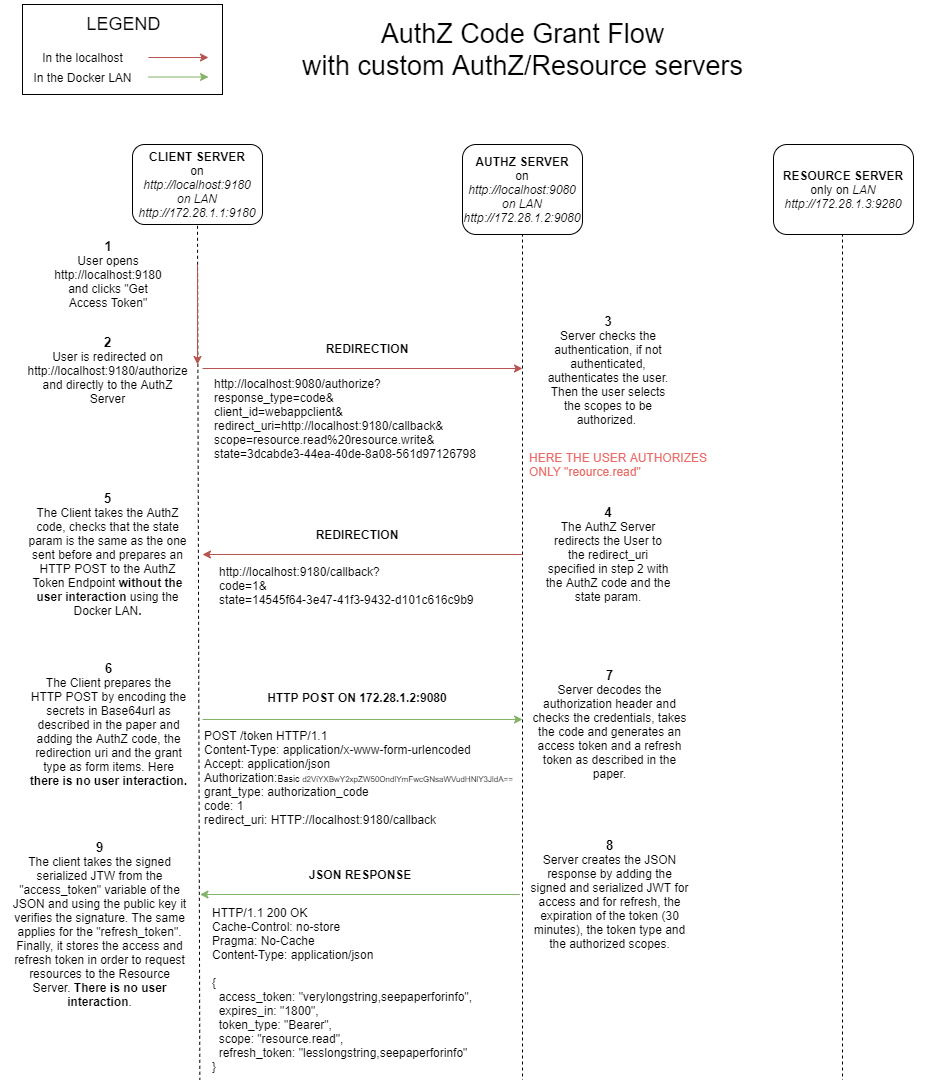
\includegraphics[width=0.85\textwidth]{figures/flow_access1.png}
    \caption{Implementation of the AuthZ Code Grant flow.}
    \label{fig:access1}
\end{figure}

\begin{enumerate}
    \item User opens \url{http://localhost:9180} and clicks "Get Access Token".
    \item User is redirected on \url{http://localhost:9180/authorize} (this starts the dedicated Servlet on the oauth2-client module, more details will follow) and directly to the AuthZ Server on \url{http://localhost:9080/authorize} (see the figure for messages format and parameters).
    \item The AuthZ Server checks the authentication of the User. If he is not authenticated, authenticates the User and finally is presented the web-page with the check-boxes of the authorization to be granted or not (\texttt{resource\_read} and \texttt{resource\_write}). 
    \item The User gives the authorization for the two scopes (or a subset of them) and the AuthZ Server redirects the User to the \texttt{redirect\_uri} specified in step 2 with the \texttt{code} (AuthZ Code) and the \texttt{state} parameter for CSRF avoidance.The URI is \url{http://localhost:9180/callback}.
    \item The oauth2-client takes the AuthZ Code, checks that the state parameter is the same as the one sent before and prepares an HTTP POST to the AuthZ Token Endpoint (\url{172.28.1.2:9080/token}) without the User interaction by using the Docker LAN.
    \item More in details, the HTTP POST is prepared by encoding the secrets in Base64url and adding the AuthZ Code, the redirection URI and the grant type as form items. There is no User interaction in this step. This step is started by the second Servlet.
    \item The AuthZ Server decodes the authorization header and checks the credentials, takes the code and generates an Access Token and a Refresh Token as later described.
    \item Furthermore, the AuthZ Server creates the JSON response by adding the signed and serialised JWT for access and for refresh, the expiration of the token (1800 seconds), the token type and the authorized scopes.
    \item Finally, the oauth2-client takes the signed serialised JTW from the \texttt{access\_token} variable of the JSON and using the public key it verifies the signature. The same applies for the \texttt{refresh\_token}. It stores the access and Refresh Token in order to request resources to the Resource Server. There is no User interaction.
\end{enumerate}



\begin{figure}[ht]
    \centering
    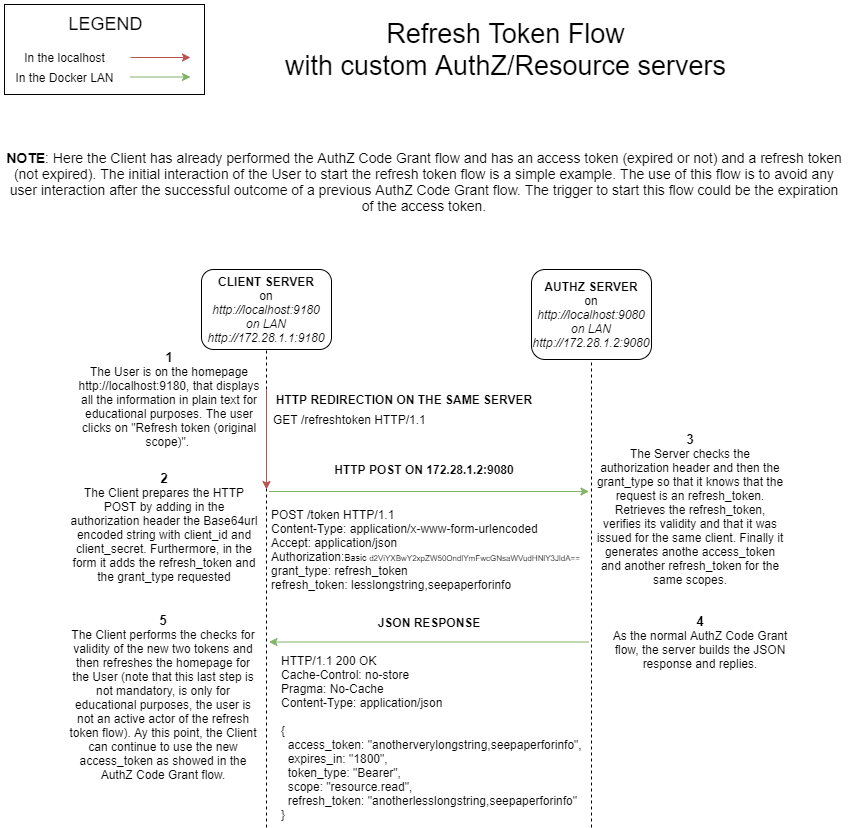
\includegraphics[width=0.85\textwidth]{figures/flow_refresh1.png}
    \caption{Implementation of the Refresh Token flow.}
    \label{fig:refresh1}
\end{figure}

The second implemented flow is the Refresh Token flow that has as objective the \texttt{access\_token} and \texttt{refresh\_token} retrieval by consuming the \texttt{refresh\_token}. The flow presumes that the oauth2-client has already performed the AuthZ Code Grant flow and has an Access Token (expired or not) and a Refresh Token (not expired). The initial interaction of the User to start the Refresh Token flow is a simple example, but the use of this flow is to avoid any User interaction after the successful outcome of a previous AuthZ Code Grant flow. For production environment, a trigger to start this flow could be the expiration of the Access Token. The steps (\myfig{\ref{fig:refresh1}}) are the following:

\begin{enumerate}
    \item The User clicks on "Refresh token (original scope)" from the homepage (\url{http://localhost:9180}). This click triggers the third Servlet of the oauth2-client module on \url{http://localhost:9180/refreshtoken}.
    \item The oauth2-client prepares the HTTP POST by adding in the authorization header the Base64url encoded string with \texttt{client\_id} and \texttt{client\_secret}. Furthermore, in the form it adds the \texttt{refresh\_token} and the \texttt{grant\_type} requested. The HTTP POST is done by using the Docker LAN on \url{172.28.1.2:9080/token}.
    \item The AuthZ Server checks the authorization header and then the \texttt{grant\_type} so that it knows that the request is a \texttt{refresh\_token}. Retrieves the \texttt{refresh\_token}, verifies its validity and that it was issued for the same Client. Finally it generates another \texttt{access\_token} and another \texttt{refresh\_token} for the same scopes.
    \item As the AuthZ Code Grant flow, the server builds the JSON response and replies.
    \item The oauth2-client performs the checks for validity of the new two tokens and then refreshes the homepage for the User (note that this last step is not mandatory, is only for educational purposes, the User is not an active actor of the Refresh Token flow). At this point, the oauth2-client can continue to use the new \texttt{access\_token}.
\end{enumerate}

I addition, it is possible to force the Refresh Token flow on a subset of the original granted scopes. For example, if the oauth2-client has authorization for "resource.read" and "resource.write", there is the possibility to force only one of them during the token refresh flow by using from the homepage "Refresh token (scope: resource.read)" or "Refresh token (scope: resource.write)". 

Taking as initial state the one with only "resource.read" authorized, if the User clicks on "Refresh token (scope: resource.write)" and the authorization that the oauth2-client has is not a subset of the requested one, the AuthZ Server will respond with an error message. In \myfig{\ref{fig:refresh3}} is showed the same Refresh Token flow forced on the scope "resource.write". 

\begin{figure}[ht]
    \centering
    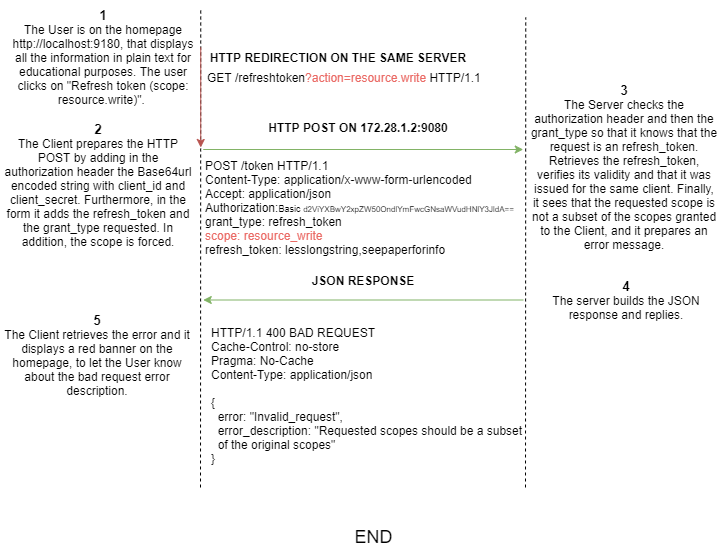
\includegraphics[width=0.85\textwidth]{figures/flow_refresh3.png}
    \caption{Implementation of the forced Refresh Token flow on "resource.write" with the message differences highlighted and BAD REQUEST error returned.}
    \label{fig:refresh3}
\end{figure}

Finally, once that the oauth2-client has the Access Token, it can perform a resource request to the Resource server (\myfig{\ref{fig:resource}}):

\begin{figure}[ht]
    \centering
    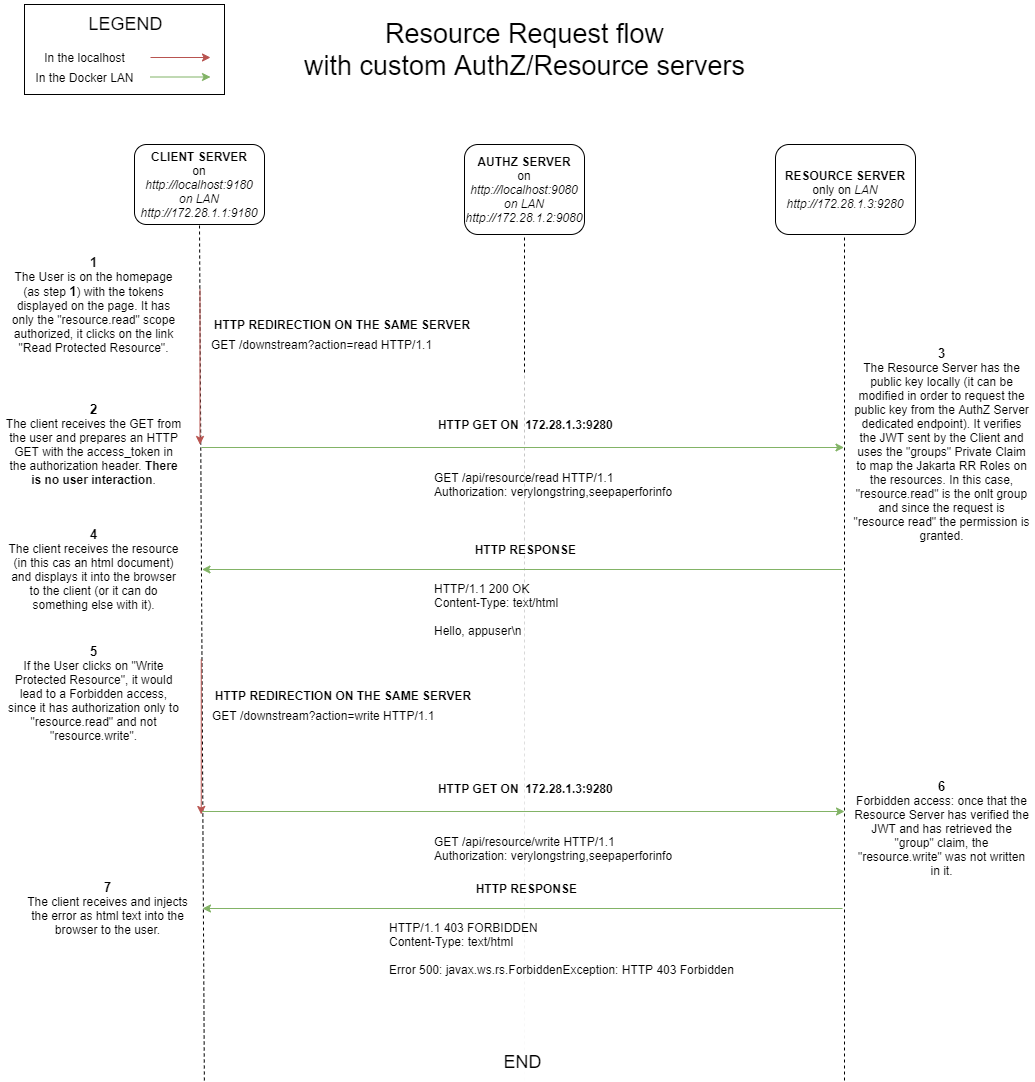
\includegraphics[width=0.85\textwidth]{figures/flow_resource.png}
    \caption{Implementation of the Resource request flow.}
    \label{fig:resource}
\end{figure}

\begin{enumerate}
    \item The User is on the homepage with the tokens displayed on the page. It has only the "resource.read" scope authorized, it clicks on the link "Read Protected Resource" (\url{http:localhost:9180/downstream?action=read})
    \item The action triggers the fourth and last Servlet of the oauth2-client. It prepares an HTTP GET to \url{172.28.1.3:9280/api/resource/read} with the \texttt{access\_token} in the authorization header. There is no User interaction.
    \item The Resource Server has the public key locally (it can be modified in order to request the public key from the AuthZ Server dedicated endpoint). It verifies the JWT sent by the Client and uses the "groups" Private Claim to map the Jakarta RR Roles on the resources. In this case, "resource.read" is the only group and, since the request is "resource read", the permission is granted. It prepares the response by adding a html-formatted string that greets the User.
    \item The oauth2-client receives the resource (in this case an html document) and displays it into the browser to the User (or it can do something else with it).
    \item If the User clicks on "Write Protected Resource", it would lead to a Forbidden access, since it has authorization only to "resource.read" and not "resource.write".
    \item Forbidden access: once that the Resource Server has verified the JWT and has retrieved the "group" claim, the "resource.write" was not written in it.
    \item The oauth2-client receives and injects the error as html text into the browser to the User.
\end{enumerate}

After this introduction on the general flows, in the following subsections is presented a detailed explanation of the implementation, divided into the three servers that compose the architecture.

% ------ SECTION B.3.1
\subsubsection{oauth2-client}
This web-server implements four Servlets\footnote{Exploit dynamic web content with Java, "[..] class that is used to extend the capabilities of servers that host applications accessed employing a request-response programming model.". Source: \url{https://docs.oracle.com/javaee/5/tutorial/doc/bnafe.html}}:

\begin{itemize}
    \item Request the authorization code from the authorization server's endpoint.
    \item Request the Access Token by consuming the authorization code.
    \item Request the Access Token by consuming the Refresh Token (\ref{accref}).
    \item Request the resource from the resource server's endpoint by consuming the Access Token.
\end{itemize}

Moreover, it uses MicroProfile Config for configuration files injection and JAX RS Client for accessing web resources. For simplicity, the \texttt{client\_id} and \texttt{client\_secret} are manually defined in the authorization server as it will be explained in the next subsection. This means that our Client must have securely stored the two secrets that, for this demo, are only one pair (since the Client is only one). In the configuration file stored in \texttt{META-INF/microprofile-config.proper-\\ties} (it must be noted that it applies the same \texttt{.template} design, as explained in the first demo), apart from the secrets, other important variables are:

\begin{itemize}
    \item \texttt{redirect\_uri}: As it was already mentioned, this is \textit{where} to receive the AuthZ code.
    \item \texttt{scope}: The permission requested by the Client.
    \item \texttt{authorization\_uri}: The Client needs to know where to send the request for the AuthZ code.
    \item \texttt{token\_uri}: As for the AuthZ URI, the Client needs to know where to send the request to exchange the code for an Access Token.
\end{itemize}

It is important though to point out that the URIs are configured for the Docker virtualized network and they need to be changed to be run without Docker.

The first Servlet implements the AuthZ code request on the AuthZ Server's endpoint and it is implemented in \textbf{AuthorizationCodeServlet.java} waiting to start on the \texttt{/authorization} endpoint of the Client. More in details, the Servlet creates and stores the \texttt{state} parameter, retrieves the information from the MicroProfile Config file and builds the URI attaching all the variables. Finally, it redirects the User to the built URI (that is on the AuthZ Server). After processing the request, the AuthZ Server will redirect back the User to the Client with the AuthZ code and the same \texttt{state} parameter on the URI \textcolor{blue}{\texttt{http://localhost:9180/callback?code=1\&-\\state=tughdj57gh5h7t7fdhgwejgg}} where the second Servlet is waiting for the AuthZ code (the Client server is on 9180, the AuthZ Server is on 9080 and the resource server on 9280).

The second Servlet starts as soon as the AuthZ Server redirects back to \texttt{/callback} with the AuthZ code and the \texttt{state} as parameters (is the only Servlet not triggered by the User in this implementation). The implementation is in \textbf{CallbackServlet.java}. First, it checks the \texttt{state} match and then it uses the received code to request an Access Token. In this case, there is no browser interaction, it is all implemented through HTTP POST and JAX RS Client: here the token endpoint requires the two secrets too in the \textit{Authentication} header, along with the code, the type of the code and the redirect URI. Now the Client has the Access Token (and the Refresh Token too) and it can access information on the resource server by using the third Servlet implemented in \textbf{DownstreamCallServlet.java} waiting on \texttt{/downstram} with two actions passed as query parameters: \textit{read} or \textit{write}. Based on the action, the Servlet calls the resource server's APIs with the Access Token in the Authorization HTTP header and receives a string if it has access or an HTTP Forbidden error if it does not.

The last Servlet is used to obtain a new Access Token starting from the Refresh Token. This is useful because it does not require the User to repeat all the flow. The Servlet is ready to start at \texttt{/refreshtoken} and, similarly to the code in \textbf{CallbackServlet.java}, it uses only JAX RS Client and HTTP POST to build the request, that has the Refresh Token, the scopes and as grant type \texttt{refresh\_token}. The Authentication header with the encoded secrets is added too. The request is posted on the same token endpoint of the AuthZ Server, but the AuthZ Server will know what to do because of the \texttt{grant\_type} parameter. If the response is 200 HTTP, the new Access Token and the new Refresh Token are stored and they can be used for the next calls.

To start the first Servlet and/or to know every parameter and token (for educational purposes), a simple homepage is built (\texttt{src/main/webapp/}\textbf{index.jsp}) that in a few words prints all the information and makes available the endpoints (by mouse click) to the User.
% ------ END SECTION B.3.1 ------

% ------ SECTION B.3.2 ------
\subsubsection{oauth2-authorization-server}
This server is the core of the \oauth\ implementation. For simplicity, a pre-configured Client credentials and a pre-configured User credentials are used, stored in

\quad \texttt{src/main/resources/data.sql.template}

It must be pointed out though that for a production environment the passwords must be hashed). 

The first important endpoint is the AuthZ endpoint that is responsible for the authentication of the User to subsequently ask for the needed permissions. The Section 3.1 of the \rfc{6749} states that "The authorization server MUST support the use of the HTTP "GET" method [\rfc{2616}] for the authorization endpoint and MAY support the use of the "POST" method as well.". In this implementation is preferred the HTTP GET method alone. Since the specification does not ask for a particular login flow, a simple login form with Jakarta EE Security can be used. The file \textbf{AuthorizationEndpoint.java} contains:

\begin{itemize}
    \item \texttt{@FormAuthenticationMechanismDefinition} to ensure that the User is logged to proceed.
    \item HTTP GET Servlet that checks the validity of the secrets, the redirect URI, the requested scope and saves all this parameters in the session and redirects the User to \textbf{authorization.jsp} from where it selects what to authorize with some check-boxes.
    \item HTTP POST Servlet that receives the User check-boxes from \textbf{authorization.jsp}, uses the saved parameters in the preceding point to populate a new AuthZ code model with the authorization code, the \texttt{client\_id}, the approved scopes, the expiration date and so on and redirects back to the Client on the \texttt{redirect\_uri} by adding to the query parameters the new code alongside the state received at the beginning for avoiding CSRF. The \texttt{redirect\_uri} must exist in the table as an authorized URI for redirections.
\end{itemize}

As mentioned before, retrieving the Access Token starting from the authorization token is an action that does not require the User nor the browser intervention. The token endpoint of the AuthZ Server, under the oauth2-client, uses JAX RS to expose the endpoint. The class \textbf{TokenEndpoint.java} implements the next step of the workflow: retrieve the Access Token. The Servlet accepts only HTTP POST and, as mentioned in the \oauth\ specification, accepted parameters mus be \texttt{application/x-www-form-urlencoded}. The first thing that the Servlet checks is the \texttt{grant\_type} that must be \texttt{authorization\_code} since this is an AuthZ Code Grant flow implementation. The second check is on \texttt{client\_id} and \texttt{client\_secret} that are in the Authorization header of the received post (this is required by the protocol to identify the Client). The two secrets are encoded into Base64url following this conversion:

\quad  \texttt{BASE64URL(client\_id:client\_secret)}

Finally, the Servlet creates the Access Token by using \textbf{AuthorizationCodeGrantTypeHandler.java}. 

Since the endpoint can and should be used for both the requests of getting an Access Token starting from an authorization code or getting an Access Token starting from a Refresh Token, the Servlet must be dynamically capable of choosing the right class instance. A possible solution is an implementation through the \textit{Contexts and Dependency Injection} (CDI). More in details, the \textbf{AuthorizationGrantTypeHandler.java} interface is created and implemented with \textbf{AuthorizationCodeGrantTypeHandler.java} for AuthZ code to Access Token and with \textbf{RefreshTokenGrantTypeHandler.java} for Refresh Token to Access Token. Each class is decorated with \texttt{@Named} that specifies for the first one the \texttt{authorization\_code} type and the second one the \texttt{refresh\_token} type. By using the decoration, in the Servlet can be written a single line of code that uses the received string (\texttt{grantType}) on the endpoint and uses it directly to load one handler or the other one:

\quad \texttt{AuthorizationGrantTypeHandler authorizationGrantTypeHandler = } 

\hspace{1cm} \texttt{authorizationGrantTypeHandlers.select(NamedLiteral.of(grantType)).get();}

To generate tokens though, it is required that the server signs them with a private RSA key. It has been used OpenSSL to generate the private key:
 
\quad \texttt{\$ openssl genpkey -algorithm RSA -out private-key.pem \textbackslash}
  
\hspace{1cm} \texttt{-pkeyopt rsa\_keygen\_bits:2048}

And the path to this key is saved in \texttt{resources/META-INF/microprofile-config.properties} to be injected into the server configuration info to be loaded directly from the code. Alongside the private key, a corresponding public key is generated:
 
\quad \texttt{\$ openssl rsa -pubout -in private-key.pem -out public-key.pem}

And stored in the same configuration file.

When the resource server receives a request with an Access Token for a resource, it has to verify it by using the public key. Another endpoint is necessary on the AuthZ Server: a JWK [\rfc{7517}] for public key distribution. This endpoint is mapped in \texttt{/jwk} and the Servlet is implemented by the class \textbf{JWKEndpoint.java}. Thanks to the Nimbus library, the code is much more simplified with both the JWT and PEM formats compatibility (by specifying the parameter \texttt{format} in the URI query).

For what concerns the authorization endpoint, it was already mentioned the existence of \textbf{AuthorizationGrantTypeHandler.java}, but how does it work? What does the endpoint returns? More in details, it uses the Nimbus JOSE library for creating a JWT token. The first thing to do is to create a JWT header and then populate the payload with some claims (like the issuer, the claimer and so on). Then, the token must be signed with the RSA Private Key. This step can be divided into two: 

\begin{itemize}
    \item The JWT is created starting from the claims and the header.
    \item The \textit{RSASSASigner} object uses the imported PEM key to sign the JWT.
\end{itemize}

Finally, the JWT is ready and it is serialised into a \textit{String}. More in details, this serialisation follows the "JWS Compact Serialization" defined in Section 7.1 of the \rfc{7515} \cite{RFC7515}:

\quad \texttt{BASE64URL(UTF8(JWS Protected Header)) || '.' ||}
  
\quad \texttt{BASE64URL(JWS Payload) || '.' ||}
  
\quad \texttt{BASE64URL(JWS Signature)}

An example of a valid serialised JWT for this implementation could be:

\begin{lstlisting}[basicstyle=\ttfamily]
  eyJ0eXAiOiJKV1QiLCJhbGciOiJSUzI1NiJ9
  .
  eyJzdWIiOiJhcHB1c2VyIiwiYXVkIjoiaHR0cDpcL1wvMTcyLjI4LjEuMzo5Mjg
  wIiwidXBuIjoiYXBwdXNlciIsIm5iZiI6MTU5Mzc5MDY1MSwic2NvcGUiOiJyZX
  NvdXJjZS5yZWFkIiwiaXNzIjoiaHR0cDpcL1wvMTcyLjI4LjEuMjo5MDgwIiwiZ
  3JvdXBzIjpbInJlc291cmNlLnJlYWQiXSwiZXhwIjoxNTkzNzkyNDUxLCJpYXQi
  OjE1OTM3OTA2NTEsImNsaWVudF9pZCI6IndlYmFwcGNsaWVudCIsImp0aSI6ImI
  3MmNiOTc2LTgxY2ItNGRjNi1hMjMwLTg2YzE2ZTE1NWQyNiJ9
  .
  pVjwobEPgfjLMdVHdBKNhwNcqpG9UytZH2wcJYtVuVFitgaDk6cWwTCCJlOLLO
  qcvtXsl4RjXavKFFGVIalQL1Smqj69u6i98VqRVn6yRiPyi8EDJeJn6Xa2BjIF
  ePjPc8EyejvM47F0LDwJO19kb-s8fcXKqEdB0zTQ8vMvb-1jgk9KlXWzsT3HxN
  rRLnpHyUAWjELVe30awwF0v9MfGPdxX64Kq62hNA2hg8TLLHXWEgU1v5eqCmdk
  sD1kyhS_cPSQLRKcXQMDPdTe1H4cnXnm8Gl_qYV885RYLx0DXqddWoiRPCLu
  5RbLr2ZXxAOSFQ8kKScmXX3BUpkiHS5afw

  
\end{lstlisting}

Where the first part of the string is the Base64url encoded of the UTF8 of the Protected Header that specifies the used algorithm and the type. The decoded string would be:

\begin{lstlisting}[basicstyle=\ttfamily]
  {
    "typ":"JWT",
    "alg":"RS256"
  }
\end{lstlisting}

The second part represents the encoded JWS Payload with all the previously built claims, decoded as:

\begin{lstlisting}[basicstyle=\ttfamily]
  {
    "sub":"appuser",
    "aud":"http://172.28.1.3:9280",
    "upn":"appuser",
    "nbf":1593790651,
    "scope":"resource.read",
    "iss":"http://172.28.1.2:9080",
    "groups":["resource.read"],
    "exp":1593792451,
    "iat":1593790651,
    "client_id":"webappclient",
    "jti":"b72cb976-81cb-4dc6-a230-86c16e155d26"
  }
\end{lstlisting}

Where, according to the \rfc{7519}\ specification \cite{RFC7519}, are defined the following Registered Claim Names:

\begin{itemize}
    \item \texttt{sub}: OPTIONAL. The principal that is the subject to the JWT.
    \item \texttt{aud}: OPTIONAL. Audience, to whom the JWT is addressed.
    \item \texttt{nbf}: OPTIONAL. Not Before, "the time before which the JWT MUST NOT be accepted for processing." \cite{RFC7519}
    \item \texttt{iss}: OPTIONAL. The issuer of the JWT.
    \item \texttt{exp}: OPTIONAL. The expiration time.
    \item \texttt{iat}: OPTIONAL. Issued At.
    \item \texttt{jti}: OPTIONAL. JWT ID, a unique identifier for the JWT.
\end{itemize}

And the following Private Claim Names designed for the demo:

\begin{itemize}
    \item \texttt{upn}: To be mapped into Jakarta EE Security \textit{CallerPrincipal}.
    \item \texttt{groups}: To be mapped into Jakarta EE \textit{Roles}.
    \item \texttt{client\_id}: The ID of the \oauth\ web-server Client.
\end{itemize}

These claims are built in the token endpoint response code in the \textbf{AbstractGrantTypeHandler.java} class. For what concerns the \texttt{refresh\_token}, the JWT is similar, with few claims and expiration of one day.
Finally, the third and last part of the JWT represents the Base64url encoded JWS Signature performed by the server on the following octets:
\begin{lstlisting}[basicstyle=\ttfamily]
  ASCII(
    BASE64URL(UTF8(JWS Protected Header)) || '.' ||
    BASE64URL(JWS Payload)
  )
\end{lstlisting}

Those octets are signed using \textit{RSASSA-PKCS1-v1\_5} with the \textit{SHA-256} hash algorithm (defined as \texttt{RS256} in the JOSE Header) by the server and finally encoded in Base64url.

The last thing to do is build the JSON response and add the elements and the serialised JWTs (refresh and Access Tokens) to return the information requested by the Client. This step is implemented in the \textbf{AuthorizationCodeGrantTypeHandler.java} class, that once it has serialised the two JWTs, it builds the response:

\begin{lstlisting}[language=bash, basicstyle=\ttfamily]
  {
    "access_token": "averylongstring,seepage46" ,
    "token_type": "Bearer",  
    "expires_in": 1800,
    "scope": "resource.read",
    "refresh_token": "smallerthanaccesstoken,lessclaims"
  }
\end{lstlisting}

A detailed diagram of the AuthZ Code Grant flow for this implementation is available in the resources as \texttt{flow\_access-token.svg}\footnote{\url{https://github.com/nopesir/oauth-hw-security-custom/releases/download/v1.0/flow_access-token.svg}}, while a detailed diagram of the Refresh Token flow is available in the resources as \texttt{flow\_refresh-token.svg}\footnote{\url{https://github.com/nopesir/oauth-hw-security-custom/releases/download/v1.0/flow_refresh-token.svg}}.
% ------ END SECTION B.3.2 ------

% ------ SECTION B.3.3 ------
\subsubsection{oauth2-resource-server}
This third and last server exposes the APIs to the Client for accessing the User's information by consuming the Access Token retrieved in the previous steps. This server uses JAX RS and MicroProfile. In particular, MicroProfile JWT is responsible for the validation and the mapping of the scopes in Jakarta roles. Thanks to these libraries, the code is pretty simple. In particular, the class \textbf{OAuth2ResourceServerApplication.java} is decorated with \texttt{@DeclareRoles} to define the scopes available and \texttt{@LoginConfig} to specify the authentication method. Finally, the class \textbf{ProtectedResource.java} represents the resource (in terms of called function) that can be personalised to return a file or any other protected information (in this example, it is a string).

It must be pointed out that even if the AuthZ Server implements the JWT endpoint, it has been chosen to add the key directly in the server's resources (to use the endpoint, the path in the configuration file has to be replaced with the endpoint of the AuthZ Server).
% ------ END SECTION B.3.3 ------
% ------ END SECTION B.3 ------

% ------ SECTION B.4 ------
\subsection{Dockerization}
To best manage, debug and deploy the two solutions, it has been chosen to dockerize the single servers. More in details, every module has its own \textbf{Dockerfile} and each demo has its \textbf{docker-compose-build.yaml} to build and run at the same time all the modules with the network configuration. Moreover, pre-built images are available on Docker Hub and a special \textbf{docker-compose.yaml} for each solution can be used to rapidly pull all the images without wasting time to build (this is mainly done for the User Guide to rapidly test and run the examples).
An important note about the example with Google/Facebook before its compilation: set \texttt{client\_id} and \texttt{client\_secret} retrieved from the registration process in Section \ref{regprocess} into the \textbf{docker-compose-build.yaml} file.

% ------ SECTION B.4.1 ------
\subsubsection{oauth-hw-security}
The first demo has two modules: the React web-app and the Spring Boot JAVA server. Each of them has its \textbf{Dockerfile}. In particular, in the hw-client, there is a two-staged docker build:

\begin{itemize}
    \item The app is built by using as base image \texttt{node:12.4.0-alpine}, producing the web-app.
    \item The web-app is copied in a simple \texttt{nginx:1.17.0-alpine} image that implements the NGINX server alongside a standard \textbf{nginx.conf}, exposing the tcp/9090 port to \texttt{localhost}.
\end{itemize}

In the hw-server module the approach is similar:

\begin{itemize}
    \item The server is built using as base image \texttt{openjdk:8-jdk-alpine} with the \texttt{mvnw} command (Maven Wrapper). Moreover, the configuration files are modified according to the different arguments passed.
    \item After that the application is packed in a \texttt{.jar}, the second stage uses \texttt{openjdk:8-jre-alpine} (a minimal image) to copy the package and run the server once that the container starts up.
\end{itemize}

These Dockerfiles are not meant to be used singularly but through \texttt{docker-compose}. The \textbf{docker-compose-build.yaml} file is responsible to use each \textbf{Dockerfile} to build the images, expose the containers in predefined ports and create some basic container network configuration. To start the local build and run the demo, the command is

\quad \texttt{\$ docker-compose -f docker-compose-build.yaml up}

That builds everything from scratch. The command needs time (there are some tasks like \texttt{npm install} that are heavy), but in the end, the two modules will be ready to test. The \textbf{docker-compose.yaml} can be used instead for a quicker run without build.

It is really important to type the same command with the \texttt{down} option when the test is finished in order to release all the residual resources of Docker.
% ------ END SECTION B.4.1 ------

% ------ SECTION B.4.2 ------
\subsubsection{oauth-hw-security-custom}
The dockerization design of the second example is identical to the first one: a \textbf{Dockerfile} for each server module that are used only by the \textbf{docker-compose-build.yaml} to entirely build and run locally the solution. The three servers use Open Liberty as server run-time, integrated with the project as Maven dependency. Moreover, some arguments are editable from the compose to correctly print personalised version of the configuration file (\eg\ for the User credentials definition or for the Client credentials definition).

The network namespace is configured as a simple LAN on \texttt{172.28.0.0/16} and the three modules are placed as follows:

\begin{itemize}
    \item oauth2-client: 172.28.1.1 on tcp/9180
    \item oauth2-authorization-server: 172.28.1.2 on tcp/9080
    \item oauth2-resource-server: 172.28.1.3 on tcp/9280
\end{itemize}

The Client and the AuthZ Server have the exposed ports on the local guest machine to be reachable from the User during the redirections of the protocol itself. The Resource Server is not accessible from the host, but only indirectly from the Client through its APIs and using the Access Token (to provide basic isolation of the resources).
\label{docker}

\begin{figure}[ht]
    \centering
    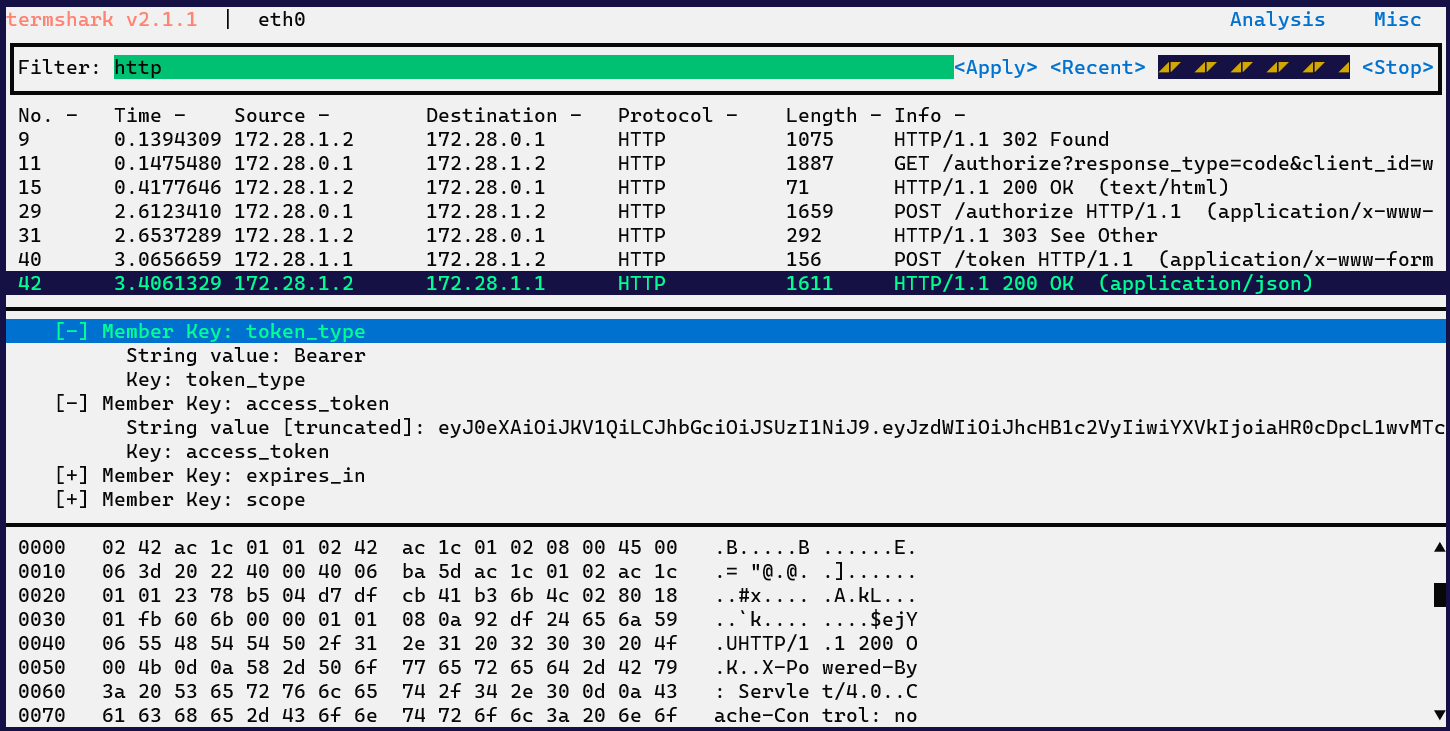
\includegraphics[width=0.9\textwidth]{figures/netshoot.png}
    \caption{Termshark running on Netshoot: caption of the Access Token JSON response from the AuthZ Server to the Client.}
    \label{fig:netshoot}
\end{figure}

Finally, to analyse and debug the messages exchanged in the Docker LAN, it has been used the \texttt{netshoot} \cite{netsh} container tool alongside \texttt{termshark} \cite{terms}. To catch all the HTTP exchanged messages from one of the three containers, simply run:

\begin{lstlisting}[basicstyle=\ttfamily]
  $ docker run -it --rm --net container:<container_name> \
     --cap-add=NET_ADMIN --cap-add=CAP_NET_RAW \
     nicolaka/netshoot termshark -i eth0 -Y http
\end{lstlisting}

As an example, if the container name of the Client (\texttt{oauth-hw-security-custom\_app-server\_1}) is set, it is possible to capture the authorization request and the JSON response of the AuthZ Server with the \texttt{access\_token} as shown in \myfig{\ref{fig:netshoot}}.
% ------ END SECTION B.4.2 ------
% ------ END SECTION B.4 ------
% ------ END SECTION B ------

% ------ BIBLIOGRAPHY ------
\begin{thebibliography}{99}
%
% Citations will be numbered according to the order
% in which they are listed in this section.
%

\bibitem{RFC6749}
D.~Hardt,
\rfc{6749} ``The OAuth 2.0 Authorization Framework'', October 2012


\bibitem{facebook}
``Manually Build a Login Flow'', \url{https://developers.facebook.com/docs/facebook-login/manually-build-a-login-flow/}

\bibitem{google1}
``Using OAuth 2.0 for Web Server Applications'', \url{https://developers.google.com/identity/protocols/oauth2/web-server}

\bibitem{google2}
``Using OAuth 2.0 to Access Google APIs'', \url{https://developers.google.com/identity/protocols/oauth2}

\bibitem{jaksec}
``Jakarta Security API documentation'', \url{https://jakarta.ee/specifications/security/1.0/apidocs/}

\bibitem{sprsec}
``Spring Security Reference'', \url{https://docs.spring.io/spring-security/site/docs/current/reference/html5/}

\bibitem{docker}
``Docker Docs'', \url{https://docs.docker.com/}

\bibitem{oauth2}
A.~Parecki, ``What is the OAuth 2.0 Authorization Code Grant Type?'', \url{https://developer.okta.com/blog/2018/04/10/oauth-authorization-code-grant-type}

\bibitem{RFC7519}
M.~Jones, J.~Bradley, N.~Sakimura, RFC-7519 ``JSON Web Token (JWT)'', November 2014

\bibitem{RFC7515}
M.~Jones, J.~Bradley, N.~Sakimura, RFC-7515 ``JSON Web Signature (JWS)'', May 2015

\bibitem{playgr}
``OAuth 2.0 Playground'', \url{https://www.oauth.com/playground/}

\bibitem{sprboot}
M.~Raible, ``Get Started with Spring Boot, OAuth 2.0, and Okta'', \url{https://developer.okta.com/blog/2017/03/21/spring-boot-oauth}

\bibitem{openid}
N.~Sakimura, J.~Bradley, M.-B.~Jones, B.~de Medeiros, C.~Mortimore, ``OpenID Connect Core 1.0 incorporating errata set 1'', \url{https://openid.net/specs/openid-connect-core-1_0.html}

\bibitem{netsh}
``Netshoot: a Docker + Kubernetes network trouble-shooting swiss-army container'', \url{https://github.com/nicolaka/netshoot}

\bibitem{terms}
``Termshark: a terminal user-interface for tshark, inspired by Wireshark.'', \url{https://github.com/gcla/termshark}

\bibitem{mastering}
Charles Bihis, ``Mastering OAuth 2.0'', 2015, chapter 9

\end{thebibliography}
% ------ END BIBLIOGRAPHY ------

\end{document}
%
% Before delivering your report, don't forget to run a spell checker,
% such as aspell (with a UK-english dictionary)
%
